% Options for packages loaded elsewhere
\PassOptionsToPackage{unicode}{hyperref}
\PassOptionsToPackage{hyphens}{url}
\PassOptionsToPackage{dvipsnames,svgnames,x11names}{xcolor}
%
\documentclass[
  11pt,
]{article}

\usepackage{amsmath,amssymb}
\usepackage{setspace}
\usepackage{iftex}
\ifPDFTeX
  \usepackage[T1]{fontenc}
  \usepackage[utf8]{inputenc}
  \usepackage{textcomp} % provide euro and other symbols
\else % if luatex or xetex
  \usepackage{unicode-math}
  \defaultfontfeatures{Scale=MatchLowercase}
  \defaultfontfeatures[\rmfamily]{Ligatures=TeX,Scale=1}
\fi
\usepackage{lmodern}
\ifPDFTeX\else  
    % xetex/luatex font selection
\fi
% Use upquote if available, for straight quotes in verbatim environments
\IfFileExists{upquote.sty}{\usepackage{upquote}}{}
\IfFileExists{microtype.sty}{% use microtype if available
  \usepackage[]{microtype}
  \UseMicrotypeSet[protrusion]{basicmath} % disable protrusion for tt fonts
}{}
\makeatletter
\@ifundefined{KOMAClassName}{% if non-KOMA class
  \IfFileExists{parskip.sty}{%
    \usepackage{parskip}
  }{% else
    \setlength{\parindent}{0pt}
    \setlength{\parskip}{6pt plus 2pt minus 1pt}}
}{% if KOMA class
  \KOMAoptions{parskip=half}}
\makeatother
\usepackage{xcolor}
\usepackage[margin=1in]{geometry}
\setlength{\emergencystretch}{3em} % prevent overfull lines
\setcounter{secnumdepth}{-\maxdimen} % remove section numbering
% Make \paragraph and \subparagraph free-standing
\makeatletter
\ifx\paragraph\undefined\else
  \let\oldparagraph\paragraph
  \renewcommand{\paragraph}{
    \@ifstar
      \xxxParagraphStar
      \xxxParagraphNoStar
  }
  \newcommand{\xxxParagraphStar}[1]{\oldparagraph*{#1}\mbox{}}
  \newcommand{\xxxParagraphNoStar}[1]{\oldparagraph{#1}\mbox{}}
\fi
\ifx\subparagraph\undefined\else
  \let\oldsubparagraph\subparagraph
  \renewcommand{\subparagraph}{
    \@ifstar
      \xxxSubParagraphStar
      \xxxSubParagraphNoStar
  }
  \newcommand{\xxxSubParagraphStar}[1]{\oldsubparagraph*{#1}\mbox{}}
  \newcommand{\xxxSubParagraphNoStar}[1]{\oldsubparagraph{#1}\mbox{}}
\fi
\makeatother

\usepackage{color}
\usepackage{fancyvrb}
\newcommand{\VerbBar}{|}
\newcommand{\VERB}{\Verb[commandchars=\\\{\}]}
\DefineVerbatimEnvironment{Highlighting}{Verbatim}{commandchars=\\\{\}}
% Add ',fontsize=\small' for more characters per line
\usepackage{framed}
\definecolor{shadecolor}{RGB}{241,243,245}
\newenvironment{Shaded}{\begin{snugshade}}{\end{snugshade}}
\newcommand{\AlertTok}[1]{\textcolor[rgb]{0.68,0.00,0.00}{#1}}
\newcommand{\AnnotationTok}[1]{\textcolor[rgb]{0.37,0.37,0.37}{#1}}
\newcommand{\AttributeTok}[1]{\textcolor[rgb]{0.40,0.45,0.13}{#1}}
\newcommand{\BaseNTok}[1]{\textcolor[rgb]{0.68,0.00,0.00}{#1}}
\newcommand{\BuiltInTok}[1]{\textcolor[rgb]{0.00,0.23,0.31}{#1}}
\newcommand{\CharTok}[1]{\textcolor[rgb]{0.13,0.47,0.30}{#1}}
\newcommand{\CommentTok}[1]{\textcolor[rgb]{0.37,0.37,0.37}{#1}}
\newcommand{\CommentVarTok}[1]{\textcolor[rgb]{0.37,0.37,0.37}{\textit{#1}}}
\newcommand{\ConstantTok}[1]{\textcolor[rgb]{0.56,0.35,0.01}{#1}}
\newcommand{\ControlFlowTok}[1]{\textcolor[rgb]{0.00,0.23,0.31}{\textbf{#1}}}
\newcommand{\DataTypeTok}[1]{\textcolor[rgb]{0.68,0.00,0.00}{#1}}
\newcommand{\DecValTok}[1]{\textcolor[rgb]{0.68,0.00,0.00}{#1}}
\newcommand{\DocumentationTok}[1]{\textcolor[rgb]{0.37,0.37,0.37}{\textit{#1}}}
\newcommand{\ErrorTok}[1]{\textcolor[rgb]{0.68,0.00,0.00}{#1}}
\newcommand{\ExtensionTok}[1]{\textcolor[rgb]{0.00,0.23,0.31}{#1}}
\newcommand{\FloatTok}[1]{\textcolor[rgb]{0.68,0.00,0.00}{#1}}
\newcommand{\FunctionTok}[1]{\textcolor[rgb]{0.28,0.35,0.67}{#1}}
\newcommand{\ImportTok}[1]{\textcolor[rgb]{0.00,0.46,0.62}{#1}}
\newcommand{\InformationTok}[1]{\textcolor[rgb]{0.37,0.37,0.37}{#1}}
\newcommand{\KeywordTok}[1]{\textcolor[rgb]{0.00,0.23,0.31}{\textbf{#1}}}
\newcommand{\NormalTok}[1]{\textcolor[rgb]{0.00,0.23,0.31}{#1}}
\newcommand{\OperatorTok}[1]{\textcolor[rgb]{0.37,0.37,0.37}{#1}}
\newcommand{\OtherTok}[1]{\textcolor[rgb]{0.00,0.23,0.31}{#1}}
\newcommand{\PreprocessorTok}[1]{\textcolor[rgb]{0.68,0.00,0.00}{#1}}
\newcommand{\RegionMarkerTok}[1]{\textcolor[rgb]{0.00,0.23,0.31}{#1}}
\newcommand{\SpecialCharTok}[1]{\textcolor[rgb]{0.37,0.37,0.37}{#1}}
\newcommand{\SpecialStringTok}[1]{\textcolor[rgb]{0.13,0.47,0.30}{#1}}
\newcommand{\StringTok}[1]{\textcolor[rgb]{0.13,0.47,0.30}{#1}}
\newcommand{\VariableTok}[1]{\textcolor[rgb]{0.07,0.07,0.07}{#1}}
\newcommand{\VerbatimStringTok}[1]{\textcolor[rgb]{0.13,0.47,0.30}{#1}}
\newcommand{\WarningTok}[1]{\textcolor[rgb]{0.37,0.37,0.37}{\textit{#1}}}

\providecommand{\tightlist}{%
  \setlength{\itemsep}{0pt}\setlength{\parskip}{0pt}}\usepackage{longtable,booktabs,array}
\usepackage{calc} % for calculating minipage widths
% Correct order of tables after \paragraph or \subparagraph
\usepackage{etoolbox}
\makeatletter
\patchcmd\longtable{\par}{\if@noskipsec\mbox{}\fi\par}{}{}
\makeatother
% Allow footnotes in longtable head/foot
\IfFileExists{footnotehyper.sty}{\usepackage{footnotehyper}}{\usepackage{footnote}}
\makesavenoteenv{longtable}
\usepackage{graphicx}
\makeatletter
\def\maxwidth{\ifdim\Gin@nat@width>\linewidth\linewidth\else\Gin@nat@width\fi}
\def\maxheight{\ifdim\Gin@nat@height>\textheight\textheight\else\Gin@nat@height\fi}
\makeatother
% Scale images if necessary, so that they will not overflow the page
% margins by default, and it is still possible to overwrite the defaults
% using explicit options in \includegraphics[width, height, ...]{}
\setkeys{Gin}{width=\maxwidth,height=\maxheight,keepaspectratio}
% Set default figure placement to htbp
\makeatletter
\def\fps@figure{htbp}
\makeatother

\usepackage{booktabs}
\usepackage{longtable}
\usepackage{array}
\usepackage{multirow}
\usepackage{wrapfig}
\usepackage{float}
\usepackage{colortbl}
\usepackage{pdflscape}
\usepackage{tabu}
\usepackage{threeparttable}
\usepackage{threeparttablex}
\usepackage[normalem]{ulem}
\usepackage{makecell}
\usepackage{xcolor}
\usepackage{booktabs}
\usepackage{longtable}
\usepackage{float}
\usepackage{amsmath}
\floatplacement{table}{H}
\floatplacement{figure}{H}
\makeatletter
\@ifpackageloaded{caption}{}{\usepackage{caption}}
\AtBeginDocument{%
\ifdefined\contentsname
  \renewcommand*\contentsname{Table of contents}
\else
  \newcommand\contentsname{Table of contents}
\fi
\ifdefined\listfigurename
  \renewcommand*\listfigurename{List of Figures}
\else
  \newcommand\listfigurename{List of Figures}
\fi
\ifdefined\listtablename
  \renewcommand*\listtablename{List of Tables}
\else
  \newcommand\listtablename{List of Tables}
\fi
\ifdefined\figurename
  \renewcommand*\figurename{Figure}
\else
  \newcommand\figurename{Figure}
\fi
\ifdefined\tablename
  \renewcommand*\tablename{Table}
\else
  \newcommand\tablename{Table}
\fi
}
\@ifpackageloaded{float}{}{\usepackage{float}}
\floatstyle{ruled}
\@ifundefined{c@chapter}{\newfloat{codelisting}{h}{lop}}{\newfloat{codelisting}{h}{lop}[chapter]}
\floatname{codelisting}{Listing}
\newcommand*\listoflistings{\listof{codelisting}{List of Listings}}
\makeatother
\makeatletter
\makeatother
\makeatletter
\@ifpackageloaded{caption}{}{\usepackage{caption}}
\@ifpackageloaded{subcaption}{}{\usepackage{subcaption}}
\makeatother

\ifLuaTeX
  \usepackage{selnolig}  % disable illegal ligatures
\fi
\usepackage{bookmark}

\IfFileExists{xurl.sty}{\usepackage{xurl}}{} % add URL line breaks if available
\urlstyle{same} % disable monospaced font for URLs
\hypersetup{
  pdftitle={Detroit Transportation Survey},
  pdfauthor={Effect Size},
  colorlinks=true,
  linkcolor={blue},
  filecolor={Maroon},
  citecolor={Blue},
  urlcolor={Blue},
  pdfcreator={LaTeX via pandoc}}


\title{Detroit Transportation Survey}
\usepackage{etoolbox}
\makeatletter
\providecommand{\subtitle}[1]{% add subtitle to \maketitle
  \apptocmd{\@title}{\par {\large #1 \par}}{}{}
}
\makeatother
\subtitle{Multi-Stage Area Probability Sample Design}
\author{Effect Size}
\date{2026-04-10}

\begin{document}
\maketitle


\setstretch{1}
\section{Sample Design}\label{sec-design}

\subsection{Design Goals}\label{design-goals}

The sample must satisfy four requirements simultaneously:

\begin{itemize}
\tightlist
\item
  Domain sample sizes: 1,000 respondents split equally (250 per group)
  across four age domains: 18--34, 35--49, 50--64, and 65+.
\item
  Self-weighting within domains: every person in a given age group has
  the same overall selection probability, \(\pi_k(d) = f_d\), so that no
  weighting adjustments are needed to compensate for unequal selection
  across PSUs within a domain.
\item
  Equal workload per PSU: the total expected number of persons to be
  contacted is the same in every sample tract, simplifying field
  management and cost control.
\item
  Two-stage selection: 40 tracts (PSUs) selected with probability
  proportional to a composite measure of size, and 1 BG (SSU) per tract,
  also selected PPS (MOS). Person-level sampling rates are specified for
  field implementation but not executed here.
\end{itemize}

\subsubsection{Packages and setup}\label{packages-and-setup}

\begin{itemize}
\tightlist
\item
  We load the packages needed for data wrangling (\texttt{tidyverse},
  \texttt{readxl}), sample selection (\texttt{sampling}), survey
  analysis (\texttt{survey}, \texttt{srvyr}, \texttt{PracTools}),
  spatial mapping (\texttt{sf}, \texttt{tigris}, \texttt{ggmap},
  \texttt{tidycensus}, \texttt{viridis}), and report formatting
  (\texttt{patchwork}, \texttt{knitr}, \texttt{scales}). The
  \texttt{tidycensus} and \texttt{ggmap} packages each require an API
  key.
\end{itemize}

\begin{Shaded}
\begin{Highlighting}[]
\NormalTok{pacman}\SpecialCharTok{::}\FunctionTok{p\_load}\NormalTok{(}
\NormalTok{  tidyverse, readxl,}
\NormalTok{  sampling,}
\NormalTok{  survey, srvyr,}
\NormalTok{  PracTools,}
\NormalTok{  sf, tigris, ggmap,}
\NormalTok{  tidycensus,}
\NormalTok{  viridis, patchwork,}
\NormalTok{  knitr, kableExtra, scales, here}
\NormalTok{)}

\FunctionTok{options}\NormalTok{(}\AttributeTok{tigris\_class =} \StringTok{"sf"}\NormalTok{, }\AttributeTok{tigris\_use\_cache =} \ConstantTok{TRUE}\NormalTok{, }\AttributeTok{scipen =} \DecValTok{999}\NormalTok{)}
\FunctionTok{set.seed}\NormalTok{(}\SpecialCharTok{{-}}\DecValTok{77}\NormalTok{)}
\end{Highlighting}
\end{Shaded}

\subsubsection{Data ingestion}\label{data-ingestion}

\begin{itemize}
\tightlist
\item
  Quarto renders in a completely fresh R session --- it does not have
  access to objects loaded in the RStudio live environment. We therefore
  read the data files using explicit paths. The \texttt{semi\_join()} on
  \texttt{tract\_fips} restricts the Wayne County records to only those
  tracts that fall inside the City of Detroit boundary.
\end{itemize}

\begin{Shaded}
\begin{Highlighting}[]
\CommentTok{\# anchor to project root regardless of where the .qmd lives}
\NormalTok{here}\SpecialCharTok{::}\FunctionTok{i\_am}\NormalTok{(}\StringTok{"inputs/Detroit\_MI.xlsx"}\NormalTok{)}

\NormalTok{input\_path   }\OtherTok{\textless{}{-}} \FunctionTok{here}\NormalTok{(}\StringTok{"inputs"}\NormalTok{)}
\NormalTok{census\_tract }\OtherTok{\textless{}{-}} \StringTok{"Census\_Tract\_FIPS\_Code\_Detroit\_MI.csv"}
\NormalTok{detroit\_mi   }\OtherTok{\textless{}{-}} \StringTok{"Detroit\_MI.xlsx"}

\NormalTok{tract\_fips }\OtherTok{\textless{}{-}} \FunctionTok{read\_csv}\NormalTok{(}
  \FunctionTok{file.path}\NormalTok{(input\_path, census\_tract),}
  \AttributeTok{col\_names =} \StringTok{"GEOID"}\NormalTok{,}
  \AttributeTok{col\_types =} \FunctionTok{cols}\NormalTok{(}\AttributeTok{GEOID =} \FunctionTok{col\_character}\NormalTok{()),}
  \AttributeTok{skip =} \DecValTok{1}\NormalTok{,}
  \AttributeTok{show\_col\_types =} \ConstantTok{FALSE}
\NormalTok{)}

\NormalTok{tract }\OtherTok{\textless{}{-}} \FunctionTok{read\_excel}\NormalTok{(}
  \FunctionTok{file.path}\NormalTok{(input\_path, detroit\_mi),}
  \AttributeTok{sheet =} \StringTok{"Tract"}
\NormalTok{) }\SpecialCharTok{|\textgreater{}}
  \FunctionTok{mutate}\NormalTok{(}\AttributeTok{Tract =} \FunctionTok{as.character}\NormalTok{(Tract)) }\SpecialCharTok{|\textgreater{}}
  \FunctionTok{semi\_join}\NormalTok{(tract\_fips, }\AttributeTok{by =} \FunctionTok{c}\NormalTok{(}\StringTok{"Tract"} \OtherTok{=} \StringTok{"GEOID"}\NormalTok{)) }\SpecialCharTok{|\textgreater{}}
  \FunctionTok{mutate}\NormalTok{(}\AttributeTok{TotPerson =} \FunctionTok{rowSums}\NormalTok{(}\FunctionTok{across}\NormalTok{(}\FunctionTok{starts\_with}\NormalTok{(}\StringTok{"Age"}\NormalTok{))))}

\NormalTok{bg }\OtherTok{\textless{}{-}} \FunctionTok{read\_excel}\NormalTok{(}
  \FunctionTok{file.path}\NormalTok{(input\_path, detroit\_mi),}
  \AttributeTok{sheet =} \StringTok{"BlockGroup"}
\NormalTok{) }\SpecialCharTok{|\textgreater{}}
  \FunctionTok{mutate}\NormalTok{(}
    \AttributeTok{BlockGroup =} \FunctionTok{as.character}\NormalTok{(BlockGroup),}
    \AttributeTok{Tract =} \FunctionTok{substr}\NormalTok{(BlockGroup, }\DecValTok{1}\NormalTok{, }\DecValTok{11}\NormalTok{)}
\NormalTok{  ) }\SpecialCharTok{|\textgreater{}}
  \FunctionTok{semi\_join}\NormalTok{(tract\_fips, }\AttributeTok{by =} \FunctionTok{c}\NormalTok{(}\StringTok{"Tract"} \OtherTok{=} \StringTok{"GEOID"}\NormalTok{))}
\end{Highlighting}
\end{Shaded}

\subsection{Target Population}\label{target-population}

The target population consists of all non-institutionalized persons aged
18 and older residing in the City of Detroit, Michigan. The 2020
Decennial Census DHC Summary File reports approximately 480,131 adults
(18+) in approximately 309,916 households across 270 eligible census
tracts. The average number of adults per household is approximately
1.55.

\subsection{Area Sampling Frame}\label{sec-frame}

\subsubsection{Data sources}\label{data-sources}

The sampling frame is constructed from two files:

\begin{itemize}
\tightlist
\item
  \textbf{Census Tract FIPS Code Detroit MI.csv}: 280 FIPS codes
  identifying Detroit census tracts, from the City of Detroit Open Data
  Portal.
\item
  \textbf{Detroit MI.xlsx}: tract- and block-group-level population data
  provided by the course instructors, originating from the 2020
  Decennial Census DHC Summary File for Wayne County, MI. It includes
  housing unit counts, total person counts, and person counts by sex and
  age from the P12 table (Sex by Age).
\end{itemize}

\subsubsection{Data cleaning}\label{data-cleaning}

\begin{itemize}
\tightlist
\item
  Tract 26163985500 (tract 9855) appears identically 25 times in the
  data with zero population in every column, likely a water body or
  uninhabited industrial zone. Since it contributes no eligible
  population, we drop all instances.
\end{itemize}

\begin{Shaded}
\begin{Highlighting}[]
\NormalTok{tract }\SpecialCharTok{|\textgreater{}}
  \FunctionTok{filter}\NormalTok{(Tract }\SpecialCharTok{==} \StringTok{"26163985500"}\NormalTok{) }\SpecialCharTok{|\textgreater{}} 
  \FunctionTok{select}\NormalTok{(}\DecValTok{1}\SpecialCharTok{:}\DecValTok{10}\NormalTok{) }\SpecialCharTok{|\textgreater{}} 
  \FunctionTok{head}\NormalTok{() }\SpecialCharTok{|\textgreater{}} 
  \FunctionTok{kable}\NormalTok{(}
    \AttributeTok{booktabs =} \ConstantTok{TRUE}\NormalTok{,}
    \AttributeTok{format =} \StringTok{"latex"}
\NormalTok{  ) }\SpecialCharTok{|\textgreater{}}
  \FunctionTok{kable\_styling}\NormalTok{(}
    \AttributeTok{latex\_options =} \FunctionTok{c}\NormalTok{(}\StringTok{"striped"}\NormalTok{, }\StringTok{"scale\_down"}\NormalTok{, }\StringTok{"hold\_position"}\NormalTok{)}
\NormalTok{  )}
\end{Highlighting}
\end{Shaded}

\begin{table}[!h]
\centering
\resizebox{\ifdim\width>\linewidth\linewidth\else\width\fi}{!}{
\begin{tabular}{llrrrrrrrr}
\toprule
Tract & NAME & TotHH & TotPerson & TotMale & MaleLT5Yrs & Male5to9Yrs & Male10to14Yrs & Male15to17Yrs & Male18to19Yrs\\
\midrule
\cellcolor{gray!10}{26163985500} & \cellcolor{gray!10}{Census Tract 9855; Wayne County; Michigan} & \cellcolor{gray!10}{0} & \cellcolor{gray!10}{0} & \cellcolor{gray!10}{0} & \cellcolor{gray!10}{0} & \cellcolor{gray!10}{0} & \cellcolor{gray!10}{0} & \cellcolor{gray!10}{0} & \cellcolor{gray!10}{\vphantom{5} 0}\\
26163985500 & Census Tract 9855; Wayne County; Michigan & 0 & 0 & 0 & 0 & 0 & 0 & 0 & \vphantom{4} 0\\
\cellcolor{gray!10}{26163985500} & \cellcolor{gray!10}{Census Tract 9855; Wayne County; Michigan} & \cellcolor{gray!10}{0} & \cellcolor{gray!10}{0} & \cellcolor{gray!10}{0} & \cellcolor{gray!10}{0} & \cellcolor{gray!10}{0} & \cellcolor{gray!10}{0} & \cellcolor{gray!10}{0} & \cellcolor{gray!10}{\vphantom{3} 0}\\
26163985500 & Census Tract 9855; Wayne County; Michigan & 0 & 0 & 0 & 0 & 0 & 0 & 0 & \vphantom{2} 0\\
\cellcolor{gray!10}{26163985500} & \cellcolor{gray!10}{Census Tract 9855; Wayne County; Michigan} & \cellcolor{gray!10}{0} & \cellcolor{gray!10}{0} & \cellcolor{gray!10}{0} & \cellcolor{gray!10}{0} & \cellcolor{gray!10}{0} & \cellcolor{gray!10}{0} & \cellcolor{gray!10}{0} & \cellcolor{gray!10}{\vphantom{1} 0}\\
\addlinespace
26163985500 & Census Tract 9855; Wayne County; Michigan & 0 & 0 & 0 & 0 & 0 & 0 & 0 & 0\\
\bottomrule
\end{tabular}}
\end{table}

\begin{Shaded}
\begin{Highlighting}[]
\CommentTok{\# drop this tract}
\NormalTok{tract }\OtherTok{\textless{}{-}}\NormalTok{ tract }\SpecialCharTok{|\textgreater{}} 
  \FunctionTok{filter}\NormalTok{(Tract }\SpecialCharTok{!=} \StringTok{"26163985500"}\NormalTok{)}

\FunctionTok{cat}\NormalTok{(}\StringTok{"We are left with"}\NormalTok{, tract }\SpecialCharTok{|\textgreater{}} \FunctionTok{nrow}\NormalTok{(), }\StringTok{"tracts"}\NormalTok{)}
\end{Highlighting}
\end{Shaded}

\begin{verbatim}
We are left with 275 tracts
\end{verbatim}

\newpage

\subsection{Frame construction (Assignment
8)}\label{frame-construction-assignment-8}

\begin{itemize}
\item
  The DHC P12 table provides 49 Sex \(\times\) Age columns per geography
  (e.g., \texttt{Male18to19Yrs}, \texttt{Female22to24Yrs}). We need to
  collapse these into the four survey age domains (18--34, 35--49,
  50--64, 65+). The \texttt{age\_patterns} named vector below is a
  single source of truth, it maps each domain label to a regex pattern
  that matches the corresponding P12 column names. If the domain
  boundaries ever change, only this vector needs updating.
\item
  The pipeline works as follows: \texttt{pivot\_longer()} reshapes all
  sex-by-age columns into rows, \texttt{map\_chr()} classifies each row
  into a domain using the regex patterns, and \texttt{pivot\_wider()}
  collapses back to one row per tract (or BG) with domain population
  counts as columns. Persons under 18 do not match any pattern and are
  removed by \texttt{filter(!is.na(AgeGroup))}.
\end{itemize}

\begin{Shaded}
\begin{Highlighting}[]
\CommentTok{\# single source of truth for age domain classification.}
\CommentTok{\# each name is the output domain label; each value is a}
\CommentTok{\# regex pattern matching the P12 column name fragments}
\CommentTok{\# that belong to that domain.}
\NormalTok{age\_patterns }\OtherTok{\textless{}{-}} \FunctionTok{c}\NormalTok{(}
  \StringTok{"Age18to34"} \OtherTok{=} \StringTok{"18to19|20Yrs|21Yrs|22to24|25to29|30to34"}\NormalTok{,}
  \StringTok{"Age35to49"} \OtherTok{=} \StringTok{"35to39|40to44|45to49"}\NormalTok{,}
  \StringTok{"Age50to64"} \OtherTok{=} \StringTok{"50to54|55to59|60to61|62to64"}\NormalTok{,}
  \StringTok{"Age65plus"} \OtherTok{=} \StringTok{"65to66|67to69|70to74|75to79|80to84|GE85"}
\NormalTok{)}

\CommentTok{\# psu frame (tract{-}level): one row per tract with}
\CommentTok{\# TotHH, TotAdult, and four age domain counts}
\NormalTok{psu\_frame }\OtherTok{\textless{}{-}}\NormalTok{ tract }\SpecialCharTok{|\textgreater{}}
  \FunctionTok{pivot\_longer}\NormalTok{(}
    \CommentTok{\# here is the regex matching}
    \AttributeTok{cols =} \FunctionTok{matches}\NormalTok{(}\StringTok{"\^{}Male[\^{}T]|\^{}Female[\^{}T]"}\NormalTok{),}
    \AttributeTok{names\_to =} \StringTok{"SexAge"}\NormalTok{, }\AttributeTok{values\_to =} \StringTok{"elements"}
\NormalTok{  ) }\SpecialCharTok{|\textgreater{}}
  \FunctionTok{select}\NormalTok{(}\SpecialCharTok{{-}}\NormalTok{TotPerson) }\SpecialCharTok{|\textgreater{}}
  \FunctionTok{mutate}\NormalTok{(}
    \CommentTok{\# classify each sex{-}by{-}age column into a domain}
    \AttributeTok{AgeGroup =} \FunctionTok{map\_chr}\NormalTok{(SexAge, }\SpecialCharTok{\textasciitilde{}}\NormalTok{ \{}
\NormalTok{      match }\OtherTok{\textless{}{-}} \FunctionTok{names}\NormalTok{(age\_patterns)[}\FunctionTok{str\_detect}\NormalTok{(.x, age\_patterns)]}
      \ControlFlowTok{if}\NormalTok{ (}\FunctionTok{length}\NormalTok{(match) }\SpecialCharTok{==} \DecValTok{0}\NormalTok{) }\ConstantTok{NA\_character\_} \ControlFlowTok{else}\NormalTok{ match}
\NormalTok{    \})}
\NormalTok{  ) }\SpecialCharTok{|\textgreater{}}
  \FunctionTok{filter}\NormalTok{(}\SpecialCharTok{!}\FunctionTok{is.na}\NormalTok{(AgeGroup)) }\SpecialCharTok{|\textgreater{}}
  \CommentTok{\# sum male + female within each domain for each tract}
  \FunctionTok{summarise}\NormalTok{(}\AttributeTok{n =} \FunctionTok{sum}\NormalTok{(elements), }\AttributeTok{.by =} \FunctionTok{c}\NormalTok{(Tract, TotHH, AgeGroup)) }\SpecialCharTok{|\textgreater{}}
  \FunctionTok{pivot\_wider}\NormalTok{(}\AttributeTok{names\_from =}\NormalTok{ AgeGroup, }\AttributeTok{values\_from =}\NormalTok{ n) }\SpecialCharTok{|\textgreater{}}
  \FunctionTok{mutate}\NormalTok{(}\AttributeTok{TotAdult =} \FunctionTok{rowSums}\NormalTok{(}\FunctionTok{across}\NormalTok{(}\FunctionTok{starts\_with}\NormalTok{(}\StringTok{"Age"}\NormalTok{)))) }\SpecialCharTok{|\textgreater{}}
  \FunctionTok{relocate}\NormalTok{(TotAdult, }\AttributeTok{.after =} \StringTok{"TotHH"}\NormalTok{)}

\CommentTok{\# ssu frame (block{-}group{-}level): same pipeline,}
\CommentTok{\# but keeps the bg and parent tract identifiers}
\NormalTok{ssu\_frame }\OtherTok{\textless{}{-}}\NormalTok{ bg }\SpecialCharTok{|\textgreater{}}
  \FunctionTok{pivot\_longer}\NormalTok{(}
    \AttributeTok{cols =} \FunctionTok{matches}\NormalTok{(}\StringTok{"\^{}Male[\^{}T]|\^{}Female[\^{}T]"}\NormalTok{),}
    \AttributeTok{names\_to =} \StringTok{"SexAge"}\NormalTok{, }\AttributeTok{values\_to =} \StringTok{"elements"}
\NormalTok{  ) }\SpecialCharTok{|\textgreater{}}
  \FunctionTok{select}\NormalTok{(}\SpecialCharTok{{-}}\NormalTok{TotPerson) }\SpecialCharTok{|\textgreater{}}
  \FunctionTok{mutate}\NormalTok{(}
    \AttributeTok{AgeGroup =} \FunctionTok{map\_chr}\NormalTok{(SexAge, }\SpecialCharTok{\textasciitilde{}}\NormalTok{ \{}
\NormalTok{      match }\OtherTok{\textless{}{-}} \FunctionTok{names}\NormalTok{(age\_patterns)[}\FunctionTok{str\_detect}\NormalTok{(.x, age\_patterns)]}
      \ControlFlowTok{if}\NormalTok{ (}\FunctionTok{length}\NormalTok{(match) }\SpecialCharTok{==} \DecValTok{0}\NormalTok{) }\ConstantTok{NA\_character\_} \ControlFlowTok{else}\NormalTok{ match}
\NormalTok{    \})}
\NormalTok{  ) }\SpecialCharTok{|\textgreater{}}
  \FunctionTok{filter}\NormalTok{(}\SpecialCharTok{!}\FunctionTok{is.na}\NormalTok{(AgeGroup)) }\SpecialCharTok{|\textgreater{}}
  \FunctionTok{summarise}\NormalTok{(}\AttributeTok{n =} \FunctionTok{sum}\NormalTok{(elements), }\AttributeTok{.by =} \FunctionTok{c}\NormalTok{(BlockGroup, Tract, TotHH, AgeGroup)) }\SpecialCharTok{|\textgreater{}}
  \FunctionTok{pivot\_wider}\NormalTok{(}\AttributeTok{names\_from =}\NormalTok{ AgeGroup, }\AttributeTok{values\_from =}\NormalTok{ n) }\SpecialCharTok{|\textgreater{}}
  \FunctionTok{mutate}\NormalTok{(}\AttributeTok{TotAdult =} \FunctionTok{rowSums}\NormalTok{(}\FunctionTok{across}\NormalTok{(}\FunctionTok{starts\_with}\NormalTok{(}\StringTok{"Age"}\NormalTok{)))) }\SpecialCharTok{|\textgreater{}}
  \FunctionTok{relocate}\NormalTok{(TotAdult, }\AttributeTok{.after =} \StringTok{"TotHH"}\NormalTok{)}

\FunctionTok{cat}\NormalTok{(}\StringTok{"psu frame:"}\NormalTok{, }\FunctionTok{nrow}\NormalTok{(psu\_frame), }\StringTok{"tracts}\SpecialCharTok{\textbackslash{}n}\StringTok{"}\NormalTok{)}
\end{Highlighting}
\end{Shaded}

\begin{verbatim}
psu frame: 275 tracts
\end{verbatim}

\begin{Shaded}
\begin{Highlighting}[]
\FunctionTok{cat}\NormalTok{(}\StringTok{"ssu frame:"}\NormalTok{, }\FunctionTok{nrow}\NormalTok{(ssu\_frame), }\StringTok{"block groups}\SpecialCharTok{\textbackslash{}n}\StringTok{"}\NormalTok{)}
\end{Highlighting}
\end{Shaded}

\begin{verbatim}
ssu frame: 627 block groups
\end{verbatim}

\subsubsection{Quality control and linking (VDK Ch. 11, Sec.
11.1)}\label{quality-control-and-linking-vdk-ch.-11-sec.-11.1}

\begin{itemize}
\item
  Before sample selection, we must verify that every unit in the frame
  can support the required workload. VDK Chapter 11 (Sec. 11.1)
  describes the quality control checks: (1) does each BG provide an
  adequate workload? (2) will any BG have a large selection probability?
  The key feasibility check from VDK p.~287 is that the within-BG
  sampling rate must not exceed 1:
  \[\pi_{k|ij}(d) = \frac{\bar{q} \, f_d}{S_{ij}} \leq 1 \quad \text{for every BG } j \text{ and domain } d\]
  where \(\bar{q}\) is the workload per BG, \(f_d\) is the domain
  sampling rate, and \(S_{ij}\) is the BG-level composite MOS. If a BG
  violates this, more persons would need to be selected from a domain
  than actually exist there.
\item
  First, we drop tracts and BGs with zero adult population (these have
  \(S_i = 0\) and would cause division-by-zero in the selection
  probability formulas). We then identify small tracts that have all
  their BGs violate the feasibility check, and combine them with
  geographic neighbors following a linking procedure introduced by Kish
  (1965) recommended in VDK Ch. 11. A few small BGs within otherwise
  large tracts also violate feasibility, but since they have near-zero
  MOS they are extremely unlikely to be selected by the PPS procedure;
  we note their existence and would apply Kish linking in the field if
  one were selected.
\end{itemize}

\begin{Shaded}
\begin{Highlighting}[]
\CommentTok{\# drop tracts with zero adult population {-}{-}{-} these are}
\CommentTok{\# ineligible areas (water, industrial, institutional)}
\NormalTok{zero\_tracts }\OtherTok{\textless{}{-}}\NormalTok{ psu\_frame }\SpecialCharTok{|\textgreater{}} \FunctionTok{filter}\NormalTok{(TotAdult }\SpecialCharTok{==} \DecValTok{0}\NormalTok{)}
\FunctionTok{cat}\NormalTok{(}\StringTok{"How many tracts to drop due to 0 adults?/n"}\NormalTok{, }
    \StringTok{"zero{-}adult tracts to drop:/n"}\NormalTok{)}
\end{Highlighting}
\end{Shaded}

\begin{verbatim}
How many tracts to drop due to 0 adults?/n zero-adult tracts to drop:/n
\end{verbatim}

\begin{Shaded}
\begin{Highlighting}[]
\NormalTok{zero\_tracts }\SpecialCharTok{|\textgreater{}} \FunctionTok{select}\NormalTok{(Tract, TotHH, TotAdult) }\SpecialCharTok{|\textgreater{}} \FunctionTok{kable}\NormalTok{()}
\end{Highlighting}
\end{Shaded}

\begin{longtable}[]{@{}lrr@{}}
\toprule\noalign{}
Tract & TotHH & TotAdult \\
\midrule\noalign{}
\endhead
\bottomrule\noalign{}
\endlastfoot
26163981800 & 1 & 0 \\
26163984200 & 0 & 0 \\
26163985800 & 0 & 0 \\
26163985900 & 0 & 0 \\
26163981700 & 0 & 0 \\
\end{longtable}

\begin{Shaded}
\begin{Highlighting}[]
\NormalTok{psu\_frame }\OtherTok{\textless{}{-}}\NormalTok{ psu\_frame }\SpecialCharTok{|\textgreater{}} \FunctionTok{filter}\NormalTok{(TotAdult }\SpecialCharTok{\textgreater{}} \DecValTok{0}\NormalTok{)}
\NormalTok{ssu\_frame }\OtherTok{\textless{}{-}}\NormalTok{ ssu\_frame }\SpecialCharTok{|\textgreater{}} \FunctionTok{filter}\NormalTok{(Tract }\SpecialCharTok{\%in\%}\NormalTok{ psu\_frame}\SpecialCharTok{$}\NormalTok{Tract)}

\CommentTok{\# also drop zero{-}adult BGs within remaining tracts}
\FunctionTok{cat}\NormalTok{(}\StringTok{"How many BGs to drop due to 0 adults?/n"}\NormalTok{,}
  \StringTok{"zero{-}adult BGs dropped:"}\NormalTok{, }\FunctionTok{sum}\NormalTok{(ssu\_frame}\SpecialCharTok{$}\NormalTok{TotAdult }\SpecialCharTok{==} \DecValTok{0}\NormalTok{), }\StringTok{"}\SpecialCharTok{\textbackslash{}n}\StringTok{"}\NormalTok{)}
\end{Highlighting}
\end{Shaded}

\begin{verbatim}
How many BGs to drop due to 0 adults?/n zero-adult BGs dropped: 9 
\end{verbatim}

\begin{Shaded}
\begin{Highlighting}[]
\NormalTok{ssu\_frame }\OtherTok{\textless{}{-}}\NormalTok{ ssu\_frame }\SpecialCharTok{|\textgreater{}} \FunctionTok{filter}\NormalTok{(TotAdult }\SpecialCharTok{\textgreater{}} \DecValTok{0}\NormalTok{)}

\FunctionTok{cat}\NormalTok{(}\StringTok{"after dropping zeros, we are left with"}\NormalTok{, }\FunctionTok{nrow}\NormalTok{(psu\_frame), }\StringTok{"tracts,"}\NormalTok{,}
    \FunctionTok{nrow}\NormalTok{(ssu\_frame), }\StringTok{"BGs}\SpecialCharTok{\textbackslash{}n}\StringTok{"}\NormalTok{)}
\end{Highlighting}
\end{Shaded}

\begin{verbatim}
after dropping zeros, we are left with 270 tracts, 612 BGs
\end{verbatim}

\hfill\break

\begin{itemize}
\tightlist
\item
  Next we compute preliminary design parameters to identify undersized
  units. The domain sampling rates under Approach A (selection-based,
  see Design Parameter section below) are
  \(f_d = n_d^{\text{select}} / N_d\) where
  \(n_d^{\text{select}} = 250 / r_d\) and \(r_d\) is the expected
  response rate from the project assignment. The workload per BG is
  \(\bar{q} = \sum_d n_d^{\text{select}} / (m \cdot \bar{n})\). The
  minimum BG MOS for feasibility is \(\bar{q} \cdot \max(f_d)\),
  corresponding to roughly 62 adults depending on age mix.
\end{itemize}

\begin{Shaded}
\begin{Highlighting}[]
\CommentTok{\# design constants from the assignment}
\NormalTok{m }\OtherTok{\textless{}{-}} \DecValTok{40}       \CommentTok{\# sample PSUs}
\NormalTok{n\_bar }\OtherTok{\textless{}{-}} \DecValTok{1}    \CommentTok{\# BGs per sample PSU}

\CommentTok{\# preliminary f\_d from the current (pre{-}linking) frame}
\NormalTok{prelim\_params }\OtherTok{\textless{}{-}} \FunctionTok{tibble}\NormalTok{(}
  \AttributeTok{domain =} \FunctionTok{c}\NormalTok{(}\StringTok{"18{-}34"}\NormalTok{, }\StringTok{"35{-}49"}\NormalTok{, }\StringTok{"50{-}64"}\NormalTok{, }\StringTok{"65+"}\NormalTok{),}
  \AttributeTok{n\_respond =} \FunctionTok{rep}\NormalTok{(}\DecValTok{250}\NormalTok{, }\DecValTok{4}\NormalTok{),}
  \CommentTok{\# given to us}
  \AttributeTok{resp\_rate =} \FunctionTok{c}\NormalTok{(}\FloatTok{0.35}\NormalTok{, }\FloatTok{0.45}\NormalTok{, }\FloatTok{0.50}\NormalTok{, }\FloatTok{0.65}\NormalTok{),}
  \AttributeTok{N\_d =} \FunctionTok{c}\NormalTok{(}\FunctionTok{sum}\NormalTok{(psu\_frame}\SpecialCharTok{$}\NormalTok{Age18to34), }\FunctionTok{sum}\NormalTok{(psu\_frame}\SpecialCharTok{$}\NormalTok{Age35to49),}
          \FunctionTok{sum}\NormalTok{(psu\_frame}\SpecialCharTok{$}\NormalTok{Age50to64), }\FunctionTok{sum}\NormalTok{(psu\_frame}\SpecialCharTok{$}\NormalTok{Age65plus))}
\NormalTok{) }\SpecialCharTok{|\textgreater{}} 
  \FunctionTok{mutate}\NormalTok{(}\AttributeTok{n\_select =}\NormalTok{ n\_respond }\SpecialCharTok{/}\NormalTok{ resp\_rate, }\AttributeTok{f\_d =}\NormalTok{ n\_select }\SpecialCharTok{/}\NormalTok{ N\_d)}

\NormalTok{f\_d\_prelim }\OtherTok{\textless{}{-}}\NormalTok{ prelim\_params}\SpecialCharTok{$}\NormalTok{f\_d}
\FunctionTok{names}\NormalTok{(f\_d\_prelim) }\OtherTok{\textless{}{-}}\NormalTok{ prelim\_params}\SpecialCharTok{$}\NormalTok{domain}
\NormalTok{q\_bar\_prelim }\OtherTok{\textless{}{-}} \FunctionTok{sum}\NormalTok{(prelim\_params}\SpecialCharTok{$}\NormalTok{n\_select) }\SpecialCharTok{/}\NormalTok{ (m }\SpecialCharTok{*}\NormalTok{ n\_bar)}

\CommentTok{\# preliminary bg{-}level mos for feasibility checks}
\NormalTok{ssu\_frame }\OtherTok{\textless{}{-}}\NormalTok{ ssu\_frame }\SpecialCharTok{|\textgreater{}}
  \FunctionTok{mutate}\NormalTok{(}\AttributeTok{MOS\_bg =}\NormalTok{ f\_d\_prelim[}\StringTok{"18{-}34"}\NormalTok{] }\SpecialCharTok{*}\NormalTok{ Age18to34 }\SpecialCharTok{+}
\NormalTok{           f\_d\_prelim[}\StringTok{"35{-}49"}\NormalTok{] }\SpecialCharTok{*}\NormalTok{ Age35to49 }\SpecialCharTok{+}
\NormalTok{           f\_d\_prelim[}\StringTok{"50{-}64"}\NormalTok{] }\SpecialCharTok{*}\NormalTok{ Age50to64 }\SpecialCharTok{+}
\NormalTok{           f\_d\_prelim[}\StringTok{"65+"}\NormalTok{] }\SpecialCharTok{*}\NormalTok{ Age65plus)}

\CommentTok{\# minimum mos needed: q\_bar * max(f\_d)}
\NormalTok{min\_mos }\OtherTok{\textless{}{-}}\NormalTok{ q\_bar\_prelim }\SpecialCharTok{*} \FunctionTok{max}\NormalTok{(f\_d\_prelim)}
\FunctionTok{cat}\NormalTok{(}\StringTok{"What is the min BG MOS for feasibility?"}\NormalTok{, }\FunctionTok{round}\NormalTok{(min\_mos, }\DecValTok{4}\NormalTok{), }\StringTok{"}\SpecialCharTok{\textbackslash{}n}\StringTok{"}\NormalTok{)}
\end{Highlighting}
\end{Shaded}

\begin{verbatim}
What is the min BG MOS for feasibility? 0.2642 
\end{verbatim}

\begin{Shaded}
\begin{Highlighting}[]
\CommentTok{\# identify violating BGs}
\NormalTok{ssu\_violations }\OtherTok{\textless{}{-}}\NormalTok{ ssu\_frame }\SpecialCharTok{|\textgreater{}} \FunctionTok{filter}\NormalTok{(MOS\_bg }\SpecialCharTok{\textless{}}\NormalTok{ min\_mos)}
\FunctionTok{cat}\NormalTok{(}\StringTok{"How many BGs are failing feasibility?"}\NormalTok{, }\FunctionTok{nrow}\NormalTok{(ssu\_violations), }\StringTok{"}\SpecialCharTok{\textbackslash{}n\textbackslash{}n}\StringTok{"}\NormalTok{)}
\end{Highlighting}
\end{Shaded}

\begin{verbatim}
How many BGs are failing feasibility? 14 
\end{verbatim}

\begin{Shaded}
\begin{Highlighting}[]
\CommentTok{\# which tracts have ALL their BGs failing? these are the}
\CommentTok{\# undersized tracts that need PSU{-}level linking}
\NormalTok{tiny\_tracts }\OtherTok{\textless{}{-}}\NormalTok{ ssu\_frame }\SpecialCharTok{|\textgreater{}}
  \FunctionTok{filter}\NormalTok{(Tract }\SpecialCharTok{\%in\%}\NormalTok{ ssu\_violations}\SpecialCharTok{$}\NormalTok{Tract) }\SpecialCharTok{|\textgreater{}}
  \FunctionTok{group\_by}\NormalTok{(Tract) }\SpecialCharTok{|\textgreater{}}
  \FunctionTok{summarise}\NormalTok{(}\AttributeTok{n\_bgs =} \FunctionTok{n}\NormalTok{(),}
            \AttributeTok{n\_fail =} \FunctionTok{sum}\NormalTok{(MOS\_bg }\SpecialCharTok{\textless{}}\NormalTok{ min\_mos), }\AttributeTok{.groups =} \StringTok{"drop"}\NormalTok{) }\SpecialCharTok{|\textgreater{}}
  \FunctionTok{filter}\NormalTok{(n\_fail }\SpecialCharTok{==}\NormalTok{ n\_bgs) }\SpecialCharTok{|\textgreater{}} 
  \FunctionTok{pull}\NormalTok{(Tract)}

\FunctionTok{cat}\NormalTok{(}\StringTok{"How many undersized tracts (all BGs fail):"}\NormalTok{, }\FunctionTok{length}\NormalTok{(tiny\_tracts), }\StringTok{"}\SpecialCharTok{\textbackslash{}n}\StringTok{"}\NormalTok{)}
\end{Highlighting}
\end{Shaded}

\begin{verbatim}
How many undersized tracts (all BGs fail): 5 
\end{verbatim}

\begin{Shaded}
\begin{Highlighting}[]
\NormalTok{psu\_frame }\SpecialCharTok{|\textgreater{}} \FunctionTok{filter}\NormalTok{(Tract }\SpecialCharTok{\%in\%}\NormalTok{ tiny\_tracts) }\SpecialCharTok{|\textgreater{}}
  \FunctionTok{select}\NormalTok{(Tract, TotHH, TotAdult) }\SpecialCharTok{|\textgreater{}} 
  \FunctionTok{kable}\NormalTok{()}
\end{Highlighting}
\end{Shaded}

\begin{longtable}[]{@{}lrr@{}}
\toprule\noalign{}
Tract & TotHH & TotAdult \\
\midrule\noalign{}
\endhead
\bottomrule\noalign{}
\endlastfoot
26163524500 & 39 & 71 \\
26163983600 & 3 & 9 \\
26163984100 & 2 & 3 \\
26163985000 & 8 & 16 \\
26163985200 & 1 & 1 \\
\end{longtable}

\newpage

\begin{itemize}
\tightlist
\item
  We combine the undersized tracts with their nearest geographic
  neighbor on the FIPS-sorted frame. The combined unit's populations and
  MOS are summed. This is a simplified version of the Kish (1965)
  linking procedure, where we sort the frame, and for each undersized
  unit, merge it forward into the next adequately-sized unit.
\end{itemize}

\begin{Shaded}
\begin{Highlighting}[]
\CommentTok{\# find the nearest non{-}tiny neighbor for each undersized tract}
\NormalTok{all\_sorted }\OtherTok{\textless{}{-}}\NormalTok{ psu\_frame }\SpecialCharTok{|\textgreater{}} \FunctionTok{arrange}\NormalTok{(Tract) }\SpecialCharTok{|\textgreater{}} \FunctionTok{pull}\NormalTok{(Tract)}
\NormalTok{non\_tiny }\OtherTok{\textless{}{-}} \FunctionTok{setdiff}\NormalTok{(all\_sorted, tiny\_tracts)}

\NormalTok{psu\_link\_map }\OtherTok{\textless{}{-}} \FunctionTok{tibble}\NormalTok{(}\AttributeTok{original =}\NormalTok{ tiny\_tracts) }\SpecialCharTok{|\textgreater{}}
  \FunctionTok{mutate}\NormalTok{(}\AttributeTok{linked\_to =} \FunctionTok{map\_chr}\NormalTok{(original, }\ControlFlowTok{function}\NormalTok{(tr) \{}
\NormalTok{    fwd }\OtherTok{\textless{}{-}}\NormalTok{ non\_tiny[non\_tiny }\SpecialCharTok{\textgreater{}}\NormalTok{ tr]}
\NormalTok{    bwd }\OtherTok{\textless{}{-}}\NormalTok{ non\_tiny[non\_tiny }\SpecialCharTok{\textless{}}\NormalTok{ tr]}
    \ControlFlowTok{if}\NormalTok{ (}\FunctionTok{length}\NormalTok{(fwd) }\SpecialCharTok{\textgreater{}} \DecValTok{0}\NormalTok{) fwd[}\DecValTok{1}\NormalTok{] }\ControlFlowTok{else} \FunctionTok{tail}\NormalTok{(bwd, }\DecValTok{1}\NormalTok{)}
\NormalTok{  \}))}

\FunctionTok{cat}\NormalTok{(}\StringTok{"We link the following PSUs:}\SpecialCharTok{\textbackslash{}n}\StringTok{"}\NormalTok{)}
\end{Highlighting}
\end{Shaded}

\begin{verbatim}
We link the following PSUs:
\end{verbatim}

\begin{Shaded}
\begin{Highlighting}[]
\NormalTok{psu\_link\_map }\SpecialCharTok{|\textgreater{}} \FunctionTok{kable}\NormalTok{()}
\end{Highlighting}
\end{Shaded}

\begin{longtable}[]{@{}ll@{}}
\toprule\noalign{}
original & linked\_to \\
\midrule\noalign{}
\endhead
\bottomrule\noalign{}
\endlastfoot
26163524500 & 26163524600 \\
26163983600 & 26163985100 \\
26163984100 & 26163985100 \\
26163985000 & 26163985100 \\
26163985200 & 26163985300 \\
\end{longtable}

\begin{Shaded}
\begin{Highlighting}[]
\CommentTok{\# assign PSU\_ID: linked tracts get their neighbor\textquotesingle{}s id}
\NormalTok{psu\_frame }\OtherTok{\textless{}{-}}\NormalTok{ psu\_frame }\SpecialCharTok{|\textgreater{}}
  \FunctionTok{mutate}\NormalTok{(}\AttributeTok{PSU\_ID =} \FunctionTok{if\_else}\NormalTok{(}
\NormalTok{    Tract }\SpecialCharTok{\%in\%}\NormalTok{ psu\_link\_map}\SpecialCharTok{$}\NormalTok{original,}
\NormalTok{    psu\_link\_map}\SpecialCharTok{$}\NormalTok{linked\_to[}\FunctionTok{match}\NormalTok{(Tract, psu\_link\_map}\SpecialCharTok{$}\NormalTok{original)],}
\NormalTok{    Tract))}

\NormalTok{ssu\_frame }\OtherTok{\textless{}{-}}\NormalTok{ ssu\_frame }\SpecialCharTok{|\textgreater{}}
  \FunctionTok{mutate}\NormalTok{(}\AttributeTok{PSU\_ID =} \FunctionTok{if\_else}\NormalTok{(}
\NormalTok{    Tract }\SpecialCharTok{\%in\%}\NormalTok{ psu\_link\_map}\SpecialCharTok{$}\NormalTok{original,}
\NormalTok{    psu\_link\_map}\SpecialCharTok{$}\NormalTok{linked\_to[}\FunctionTok{match}\NormalTok{(Tract, psu\_link\_map}\SpecialCharTok{$}\NormalTok{original)],}
\NormalTok{    Tract))}

\CommentTok{\# aggregate to composite psu level}
\NormalTok{psu\_frame }\OtherTok{\textless{}{-}}\NormalTok{ psu\_frame }\SpecialCharTok{|\textgreater{}}
  \FunctionTok{group\_by}\NormalTok{(PSU\_ID) }\SpecialCharTok{|\textgreater{}}
  \FunctionTok{reframe}\NormalTok{(}\AttributeTok{n\_tracts =} \FunctionTok{n}\NormalTok{(), }\AttributeTok{TotHH =} \FunctionTok{sum}\NormalTok{(TotHH), }\AttributeTok{TotAdult =} \FunctionTok{sum}\NormalTok{(TotAdult),}
            \AttributeTok{Age18to34 =} \FunctionTok{sum}\NormalTok{(Age18to34), }\AttributeTok{Age35to49 =} \FunctionTok{sum}\NormalTok{(Age35to49),}
            \AttributeTok{Age50to64 =} \FunctionTok{sum}\NormalTok{(Age50to64), }\AttributeTok{Age65plus =} \FunctionTok{sum}\NormalTok{(Age65plus)) }\SpecialCharTok{|\textgreater{}}
  \FunctionTok{rename}\NormalTok{(}\AttributeTok{Tract =}\NormalTok{ PSU\_ID)}

\CommentTok{\# update ssu\_frame: drop old Tract (original parent tract id),}
\CommentTok{\# replace with PSU\_ID (the linked{-}to tract), and drop stale MOS}
\NormalTok{ssu\_frame }\OtherTok{\textless{}{-}}\NormalTok{ ssu\_frame }\SpecialCharTok{|\textgreater{}}
  \FunctionTok{select}\NormalTok{(}\SpecialCharTok{{-}}\NormalTok{Tract, }\SpecialCharTok{{-}}\NormalTok{MOS\_bg) }\SpecialCharTok{|\textgreater{}}
  \FunctionTok{rename}\NormalTok{(}\AttributeTok{Tract =}\NormalTok{ PSU\_ID)}

\FunctionTok{cat}\NormalTok{(}\StringTok{"How many PSU after linking?"}\NormalTok{, }\FunctionTok{nrow}\NormalTok{(psu\_frame), }\StringTok{"PSUs}\SpecialCharTok{\textbackslash{}n}\StringTok{"}\NormalTok{)}
\end{Highlighting}
\end{Shaded}

\begin{verbatim}
How many PSU after linking? 265 PSUs
\end{verbatim}

\begin{Shaded}
\begin{Highlighting}[]
\FunctionTok{cat}\NormalTok{(}\StringTok{"How many combined PSUs?"}\NormalTok{, }\FunctionTok{sum}\NormalTok{(psu\_frame}\SpecialCharTok{$}\NormalTok{n\_tracts }\SpecialCharTok{\textgreater{}} \DecValTok{1}\NormalTok{), }\StringTok{"}\SpecialCharTok{\textbackslash{}n}\StringTok{"}\NormalTok{)}
\end{Highlighting}
\end{Shaded}

\begin{verbatim}
How many combined PSUs? 3 
\end{verbatim}

\newpage

\subsection{Design parameters (Assignment 8)}\label{sec-params}

\begin{itemize}
\item
  The composite MOS method (VDK Sec. 10.5) requires domain sampling
  rates \(f_d = n_d / N_d\), where \(n_d\) is the desired domain sample
  size and \(N_d\) is the domain population. VDK p.~282 defines this
  notation. There are two conventions for what \(n_d\) means:

  \begin{itemize}
  \item
    \textbf{Approach A (selection-based)}:
    \(n_d = n_d^{\text{select}} = 250 / r_d\), the number of persons to
    \emph{contact} in each domain, inflated for the expected
    non-response rate \(r_d\). This builds NR into the MOS so the design
    directly yields enough selections to produce 250 respondents per
    domain after expected losses.
  \item
    \textbf{Approach B (respondent-based, VDK Ch. 11 pattern)}:
    \(n_d = 250\), the respondent target. This is how the Anne Arundel
    County example in VDK Table 11.1 is set up. NR inflation is then
    applied at the person-selection stage in the field rather than in
    the MOS.
  \end{itemize}
\item
  Under Approach A, the workload per BG is
  \(\bar{q} = \sum_d n_d^{\text{select}} / (m \cdot \bar{n}) \approx 53.9\)
  persons to contact. Under Approach B, \(\bar{q} = 1000 / 40 = 25\)
  respondents. We proceed with \textbf{Approach A} because it keeps all
  selection probabilities self-contained at the design stage --- field
  teams simply apply the rates; no additional NR inflation is needed.
\end{itemize}

\begin{Shaded}
\begin{Highlighting}[]
\CommentTok{\# recompute N\_d from the cleaned, linked frame}
\NormalTok{N\_d }\OtherTok{\textless{}{-}} \FunctionTok{c}\NormalTok{(}\FunctionTok{sum}\NormalTok{(psu\_frame}\SpecialCharTok{$}\NormalTok{Age18to34), }\FunctionTok{sum}\NormalTok{(psu\_frame}\SpecialCharTok{$}\NormalTok{Age35to49),}
         \FunctionTok{sum}\NormalTok{(psu\_frame}\SpecialCharTok{$}\NormalTok{Age50to64), }\FunctionTok{sum}\NormalTok{(psu\_frame}\SpecialCharTok{$}\NormalTok{Age65plus))}

\CommentTok{\# approach A: selection{-}based f\_d}
\NormalTok{design\_params }\OtherTok{\textless{}{-}} \FunctionTok{tibble}\NormalTok{(}
  \AttributeTok{domain =} \FunctionTok{c}\NormalTok{(}\StringTok{"18{-}34"}\NormalTok{, }\StringTok{"35{-}49"}\NormalTok{, }\StringTok{"50{-}64"}\NormalTok{, }\StringTok{"65+"}\NormalTok{),}
  \AttributeTok{n\_respond =} \FunctionTok{rep}\NormalTok{(}\DecValTok{250}\NormalTok{, }\DecValTok{4}\NormalTok{),}
  \AttributeTok{resp\_rate =} \FunctionTok{c}\NormalTok{(}\FloatTok{0.35}\NormalTok{, }\FloatTok{0.45}\NormalTok{, }\FloatTok{0.50}\NormalTok{, }\FloatTok{0.65}\NormalTok{),}
  \AttributeTok{N\_d =}\NormalTok{ N\_d}
\NormalTok{) }\SpecialCharTok{|\textgreater{}} 
  \FunctionTok{mutate}\NormalTok{(}
  \AttributeTok{n\_select =}\NormalTok{ n\_respond }\SpecialCharTok{/}\NormalTok{ resp\_rate, }\CommentTok{\# inflate for NR}
  \AttributeTok{f\_d =}\NormalTok{ n\_select }\SpecialCharTok{/}\NormalTok{ N\_d }\CommentTok{\# domain sampling rate}
\NormalTok{)}

\FunctionTok{cat}\NormalTok{(}\StringTok{"Design parameters (Approach A):}\SpecialCharTok{\textbackslash{}n}\StringTok{"}\NormalTok{)}
\end{Highlighting}
\end{Shaded}

\begin{verbatim}
Design parameters (Approach A):
\end{verbatim}

\begin{Shaded}
\begin{Highlighting}[]
\NormalTok{design\_params }\SpecialCharTok{|\textgreater{}} 
  \FunctionTok{mutate}\NormalTok{(}\FunctionTok{across}\NormalTok{(}\FunctionTok{where}\NormalTok{(is.numeric), }\SpecialCharTok{\textasciitilde{}} \FunctionTok{round}\NormalTok{(.x, }\DecValTok{6}\NormalTok{))) }\SpecialCharTok{|\textgreater{}} 
  \FunctionTok{kable}\NormalTok{()}
\end{Highlighting}
\end{Shaded}

\begin{longtable}[]{@{}lrrrrr@{}}
\toprule\noalign{}
domain & n\_respond & resp\_rate & N\_d & n\_select & f\_d \\
\midrule\noalign{}
\endhead
\bottomrule\noalign{}
\endlastfoot
18-34 & 250 & 0.35 & 161357 & 714.2857 & 0.004427 \\
35-49 & 250 & 0.45 & 113272 & 555.5556 & 0.004905 \\
50-64 & 250 & 0.50 & 117763 & 500.0000 & 0.004246 \\
65+ & 250 & 0.65 & 87739 & 384.6154 & 0.004384 \\
\end{longtable}

\begin{Shaded}
\begin{Highlighting}[]
\CommentTok{\# extract as named vector}
\NormalTok{f\_d }\OtherTok{\textless{}{-}}\NormalTok{ design\_params}\SpecialCharTok{$}\NormalTok{f\_d}
\FunctionTok{names}\NormalTok{(f\_d) }\OtherTok{\textless{}{-}}\NormalTok{ design\_params}\SpecialCharTok{$}\NormalTok{domain}
\NormalTok{total\_select }\OtherTok{\textless{}{-}} \FunctionTok{sum}\NormalTok{(design\_params}\SpecialCharTok{$}\NormalTok{n\_select)}
\NormalTok{q\_bar }\OtherTok{\textless{}{-}}\NormalTok{ total\_select }\SpecialCharTok{/}\NormalTok{ (m }\SpecialCharTok{*}\NormalTok{ n\_bar)}

\FunctionTok{cat}\NormalTok{(}\StringTok{"Total selections (S):"}\NormalTok{, }\FunctionTok{round}\NormalTok{(total\_select, }\DecValTok{1}\NormalTok{), }\StringTok{"}\SpecialCharTok{\textbackslash{}n}\StringTok{"}\NormalTok{)}
\end{Highlighting}
\end{Shaded}

\begin{verbatim}
Total selections (S): 2154.5 
\end{verbatim}

\begin{Shaded}
\begin{Highlighting}[]
\FunctionTok{cat}\NormalTok{(}\StringTok{"Workload per BG (q\_bar):"}\NormalTok{, }\FunctionTok{round}\NormalTok{(q\_bar, }\DecValTok{1}\NormalTok{), }\StringTok{"persons}\SpecialCharTok{\textbackslash{}n}\StringTok{"}\NormalTok{)}
\end{Highlighting}
\end{Shaded}

\begin{verbatim}
Workload per BG (q_bar): 53.9 persons
\end{verbatim}

\newpage

\subsection{Composite MOS (VDK Eq. 10.1, Assignment 8)}\label{sec-mos}

\begin{itemize}
\item
  The composite measure of size for PSU \(i\) is defined as (VDK Eq.
  10.1, p.~282): \[S_i = \sum_{d=1}^{D} f_d \cdot N_i(d)\] This quantity
  represents the expected sample size from PSU \(i\) if the desired
  domain sampling rates were applied to its domain populations. The
  total MOS across all PSUs equals the total desired sample size:
  \(S = \sum_{i \in U} S_i = \sum_d f_d N_d = n^{\text{select}}\) (VDK
  p.~282).
\item
  PSU selection probabilities are proportional to \(S_i\) (VDK p.~282):
  \[\pi_i = \frac{m \cdot S_i}{S}\]
\item
  For the three-stage extension (VDK p.~286), the BG-level composite MOS
  is \(S_{ij} = \sum_d f_d \cdot Q_{ij}(d)\) where \(Q_{ij}(d)\) is the
  population of domain \(d\) in BG \(j\) of tract \(i\). The BG
  conditional selection probability is
  \(\pi_{j|i} = \bar{n} \cdot S_{ij} / S_i\) (VDK p.~286). Note that
  since \(\bar{n} = 1\) in our design, \(\pi_{j|i} = S_{ij} / S_i\).
\item
  The within-BG person sampling rate for domain \(d\) is (VDK p.~288):
  \[\pi_{k|ij}(d) = \frac{\bar{q} \, f_d}{S_{ij}}\] The self-weighting
  property then follows algebraically (VDK p.~286):
  \[\pi_i \cdot \pi_{j|i} \cdot \pi_{k|ij}(d) = \frac{m \, S_i}{S} \cdot \frac{\bar{n} \, S_{ij}}{S_i} \cdot \frac{\bar{q} \, f_d}{S_{ij}} = \frac{m \, \bar{n} \, \bar{q}}{S} \, f_d = f_d\]
  since \(S = m \cdot \bar{n} \cdot \bar{q}\) (VDK p.~286).
\item
  The workload is constant in every BG (VDK p.~287):
  \(\sum_d q^*_{ij}(d) = \bar{q}\), where
  \(q^*_{ij}(d) = \bar{q} \, f_d \, Q_{ij}(d) / S_{ij}\) is the expected
  number of domain-\(d\) selections in BG \(ij\) (analogous to VDK Eq.
  10.2 at the SSU level).
\end{itemize}

\begin{Shaded}
\begin{Highlighting}[]
\CommentTok{\# psu{-}level composite mos and selection probabilities}
\CommentTok{\# named vector ensures correct column{-}to{-}rate alignment}
\NormalTok{domain\_cols }\OtherTok{\textless{}{-}} \FunctionTok{c}\NormalTok{(}\StringTok{"Age18to34"}\NormalTok{, }\StringTok{"Age35to49"}\NormalTok{, }\StringTok{"Age50to64"}\NormalTok{, }\StringTok{"Age65plus"}\NormalTok{)}

\NormalTok{psu\_frame }\OtherTok{\textless{}{-}}\NormalTok{ psu\_frame }\SpecialCharTok{|\textgreater{}}
  \FunctionTok{mutate}\NormalTok{(}
    \AttributeTok{MOS =} \FunctionTok{rowSums}\NormalTok{(}\FunctionTok{across}\NormalTok{(}\FunctionTok{all\_of}\NormalTok{(domain\_cols)) }\SpecialCharTok{*}\NormalTok{ f\_d),}
    \AttributeTok{pi\_i =}\NormalTok{ m }\SpecialCharTok{*}\NormalTok{ MOS }\SpecialCharTok{/} \FunctionTok{sum}\NormalTok{(MOS))}

\NormalTok{S\_total }\OtherTok{\textless{}{-}} \FunctionTok{sum}\NormalTok{(psu\_frame}\SpecialCharTok{$}\NormalTok{MOS)}
\FunctionTok{cat}\NormalTok{(}\StringTok{"S ="}\NormalTok{, }\FunctionTok{round}\NormalTok{(S\_total, }\DecValTok{2}\NormalTok{),}
    \StringTok{"| should equal total\_select ="}\NormalTok{, }\FunctionTok{round}\NormalTok{(total\_select, }\DecValTok{2}\NormalTok{), }\StringTok{"}\SpecialCharTok{\textbackslash{}n}\StringTok{"}\NormalTok{)}
\end{Highlighting}
\end{Shaded}

\begin{verbatim}
S = 2156.13 | should equal total_select = 2154.46 
\end{verbatim}

\begin{Shaded}
\begin{Highlighting}[]
\FunctionTok{cat}\NormalTok{(}\StringTok{"pi\_i range:"}\NormalTok{, }\FunctionTok{round}\NormalTok{(}\FunctionTok{range}\NormalTok{(psu\_frame}\SpecialCharTok{$}\NormalTok{pi\_i), }\DecValTok{4}\NormalTok{), }\StringTok{"}\SpecialCharTok{\textbackslash{}n}\StringTok{"}\NormalTok{)}
\end{Highlighting}
\end{Shaded}

\begin{verbatim}
pi_i range: 0.0136 0.3692 
\end{verbatim}

\begin{Shaded}
\begin{Highlighting}[]
\FunctionTok{cat}\NormalTok{(}\StringTok{"any pi\_i \textgreater{} 1?"}\NormalTok{, }\FunctionTok{any}\NormalTok{(psu\_frame}\SpecialCharTok{$}\NormalTok{pi\_i }\SpecialCharTok{\textgreater{}} \DecValTok{1}\NormalTok{), }\StringTok{"}\SpecialCharTok{\textbackslash{}n}\StringTok{"}\NormalTok{)}
\end{Highlighting}
\end{Shaded}

\begin{verbatim}
any pi_i > 1? FALSE 
\end{verbatim}

\begin{Shaded}
\begin{Highlighting}[]
\CommentTok{\# bg{-}level composite mos}
\NormalTok{ssu\_frame }\OtherTok{\textless{}{-}}\NormalTok{ ssu\_frame }\SpecialCharTok{|\textgreater{}}
  \FunctionTok{mutate}\NormalTok{(}\AttributeTok{MOS\_bg =}\NormalTok{ f\_d[}\StringTok{"18{-}34"}\NormalTok{] }\SpecialCharTok{*}\NormalTok{ Age18to34 }\SpecialCharTok{+}\NormalTok{ f\_d[}\StringTok{"35{-}49"}\NormalTok{] }\SpecialCharTok{*}\NormalTok{ Age35to49 }\SpecialCharTok{+}
\NormalTok{           f\_d[}\StringTok{"50{-}64"}\NormalTok{] }\SpecialCharTok{*}\NormalTok{ Age50to64 }\SpecialCharTok{+}\NormalTok{ f\_d[}\StringTok{"65+"}\NormalTok{] }\SpecialCharTok{*}\NormalTok{ Age65plus)}
\end{Highlighting}
\end{Shaded}

\subsection{VDK 10.1 verification table}\label{sec-vdk-verify}

\begin{itemize}
\item
  Following the spreadsheet layout in VDK Example 10.1 (Table 10.1,
  p.~284), we verify four properties at the PSU level. These are the
  same checks Kevin performed in Assignment 8 (VDK Exercise 10.2) using
  the two-domain example, extended here to four domains and applied to
  our Detroit frame.

  \begin{enumerate}
  \def\labelenumi{\arabic{enumi}.}
  \tightlist
  \item
    \textbf{Feasibility}: \(f_d \leq S_i / \bar{q}\) for every domain,
    equivalently \(\bar{q} f_d / S_i \leq 1\).
  \item
    \textbf{Expected domain sample sizes}:
    \(n^*_i(d) = \bar{q} \, f_d \, N_i(d) / S_i\) (VDK Eq. 10.2 adapted
    to our notation).
  \item
    \textbf{Constant workload}: \(\sum_d n^*_i(d) = \bar{q}\) for every
    PSU.
  \item
    \textbf{Self-weighting}: \(\pi_i \cdot \pi_{k|i}(d) = f_d\), where
    \(\pi_{k|i}(d) = \bar{q} \, f_d / S_i\) is the within-PSU person
    rate.
  \end{enumerate}
\end{itemize}

\begin{Shaded}
\begin{Highlighting}[]
\NormalTok{vdk\_table }\OtherTok{\textless{}{-}}\NormalTok{ psu\_frame }\SpecialCharTok{|\textgreater{}}
  \FunctionTok{mutate}\NormalTok{(}
    \CommentTok{\# within{-}psu domain rates (= q\_bar * f\_d / S\_i)}
    \AttributeTok{rate\_18\_34  =}\NormalTok{ q\_bar }\SpecialCharTok{*}\NormalTok{ f\_d[}\StringTok{"18{-}34"}\NormalTok{]  }\SpecialCharTok{/}\NormalTok{ MOS,}
    \AttributeTok{rate\_35\_49  =}\NormalTok{ q\_bar }\SpecialCharTok{*}\NormalTok{ f\_d[}\StringTok{"35{-}49"}\NormalTok{]  }\SpecialCharTok{/}\NormalTok{ MOS,}
    \AttributeTok{rate\_50\_64  =}\NormalTok{ q\_bar }\SpecialCharTok{*}\NormalTok{ f\_d[}\StringTok{"50{-}64"}\NormalTok{]  }\SpecialCharTok{/}\NormalTok{ MOS,}
    \AttributeTok{rate\_65plus =}\NormalTok{ q\_bar }\SpecialCharTok{*}\NormalTok{ f\_d[}\StringTok{"65+"}\NormalTok{]    }\SpecialCharTok{/}\NormalTok{ MOS,}
    \CommentTok{\# (1) feasibility: all rates must be \textless{}= 1}
    \AttributeTok{feas\_18\_34 =}\NormalTok{ rate\_18\_34 }\SpecialCharTok{\textless{}=} \DecValTok{1}\NormalTok{, }\AttributeTok{feas\_35\_49 =}\NormalTok{ rate\_35\_49 }\SpecialCharTok{\textless{}=} \DecValTok{1}\NormalTok{,}
    \AttributeTok{feas\_50\_64 =}\NormalTok{ rate\_50\_64 }\SpecialCharTok{\textless{}=} \DecValTok{1}\NormalTok{, }\AttributeTok{feas\_65plus =}\NormalTok{ rate\_65plus }\SpecialCharTok{\textless{}=} \DecValTok{1}\NormalTok{,}
    \CommentTok{\# (2) expected domain sample sizes}
    \AttributeTok{exp\_n\_18\_34  =}\NormalTok{ rate\_18\_34 }\SpecialCharTok{*}\NormalTok{ Age18to34,}
    \AttributeTok{exp\_n\_35\_49  =}\NormalTok{ rate\_35\_49 }\SpecialCharTok{*}\NormalTok{ Age35to49,}
    \AttributeTok{exp\_n\_50\_64  =}\NormalTok{ rate\_50\_64 }\SpecialCharTok{*}\NormalTok{ Age50to64,}
    \AttributeTok{exp\_n\_65plus =}\NormalTok{ rate\_65plus }\SpecialCharTok{*}\NormalTok{ Age65plus,}
    \CommentTok{\# (3) total workload per psu}
    \AttributeTok{exp\_workload =}\NormalTok{ exp\_n\_18\_34 }\SpecialCharTok{+}\NormalTok{ exp\_n\_35\_49 }\SpecialCharTok{+}\NormalTok{ exp\_n\_50\_64 }\SpecialCharTok{+}\NormalTok{ exp\_n\_65plus,}
    \CommentTok{\# (4) self{-}weighting: pi\_i * rate\_d should equal f\_d}
    \AttributeTok{sw\_18\_34 =}\NormalTok{ pi\_i }\SpecialCharTok{*}\NormalTok{ rate\_18\_34, }\AttributeTok{sw\_35\_49 =}\NormalTok{ pi\_i }\SpecialCharTok{*}\NormalTok{ rate\_35\_49,}
    \AttributeTok{sw\_50\_64 =}\NormalTok{ pi\_i }\SpecialCharTok{*}\NormalTok{ rate\_50\_64, }\AttributeTok{sw\_65plus =}\NormalTok{ pi\_i }\SpecialCharTok{*}\NormalTok{ rate\_65plus)}

\FunctionTok{cat}\NormalTok{(}\StringTok{"(1) all within{-}psu rates \textless{}= 1?}\SpecialCharTok{\textbackslash{}n}\StringTok{"}\NormalTok{)}
\end{Highlighting}
\end{Shaded}

\begin{verbatim}
(1) all within-psu rates <= 1?
\end{verbatim}

\begin{Shaded}
\begin{Highlighting}[]
\NormalTok{vdk\_table }\SpecialCharTok{|\textgreater{}} \FunctionTok{summarise}\NormalTok{(}\FunctionTok{across}\NormalTok{(}\FunctionTok{starts\_with}\NormalTok{(}\StringTok{"feas"}\NormalTok{), }\SpecialCharTok{\textasciitilde{}} \FunctionTok{all}\NormalTok{(.x))) }\SpecialCharTok{|\textgreater{}} \FunctionTok{kable}\NormalTok{()}
\end{Highlighting}
\end{Shaded}

\begin{longtable}[]{@{}llll@{}}
\toprule\noalign{}
feas\_18\_34 & feas\_35\_49 & feas\_50\_64 & feas\_65plus \\
\midrule\noalign{}
\endhead
\bottomrule\noalign{}
\endlastfoot
TRUE & TRUE & TRUE & TRUE \\
\end{longtable}

\begin{Shaded}
\begin{Highlighting}[]
\FunctionTok{cat}\NormalTok{(}\StringTok{"}\SpecialCharTok{\textbackslash{}n}\StringTok{(3) workload per psu (should all ="}\NormalTok{, }\FunctionTok{round}\NormalTok{(q\_bar, }\DecValTok{2}\NormalTok{), }\StringTok{"):}\SpecialCharTok{\textbackslash{}n}\StringTok{"}\NormalTok{)}
\end{Highlighting}
\end{Shaded}

\begin{verbatim}

(3) workload per psu (should all = 53.86 ):
\end{verbatim}

\begin{Shaded}
\begin{Highlighting}[]
\FunctionTok{summary}\NormalTok{(vdk\_table}\SpecialCharTok{$}\NormalTok{exp\_workload)}
\end{Highlighting}
\end{Shaded}

\begin{verbatim}
   Min. 1st Qu.  Median    Mean 3rd Qu.    Max. 
  50.70   53.52   53.86   53.81   53.99   55.79 
\end{verbatim}

\begin{Shaded}
\begin{Highlighting}[]
\FunctionTok{cat}\NormalTok{(}\StringTok{"}\SpecialCharTok{\textbackslash{}n}\StringTok{(4) self{-}weighting check (first 5 PSUs):}\SpecialCharTok{\textbackslash{}n}\StringTok{"}\NormalTok{)}
\end{Highlighting}
\end{Shaded}

\begin{verbatim}

(4) self-weighting check (first 5 PSUs):
\end{verbatim}

\begin{Shaded}
\begin{Highlighting}[]
\FunctionTok{cat}\NormalTok{(}\StringTok{"target f\_d:"}\NormalTok{, }\FunctionTok{round}\NormalTok{(f\_d, }\DecValTok{6}\NormalTok{), }\StringTok{"}\SpecialCharTok{\textbackslash{}n}\StringTok{"}\NormalTok{)}
\end{Highlighting}
\end{Shaded}

\begin{verbatim}
target f_d: 0.004427 0.004905 0.004246 0.004384 
\end{verbatim}

\begin{Shaded}
\begin{Highlighting}[]
\NormalTok{vdk\_table }\SpecialCharTok{|\textgreater{}} \FunctionTok{select}\NormalTok{(Tract, }\FunctionTok{starts\_with}\NormalTok{(}\StringTok{"sw\_"}\NormalTok{)) }\SpecialCharTok{|\textgreater{}}
  \FunctionTok{slice\_head}\NormalTok{(}\AttributeTok{n =} \DecValTok{5}\NormalTok{) }\SpecialCharTok{|\textgreater{}}
  \FunctionTok{mutate}\NormalTok{(}\FunctionTok{across}\NormalTok{(}\FunctionTok{where}\NormalTok{(is.numeric), }\SpecialCharTok{\textasciitilde{}} \FunctionTok{round}\NormalTok{(.x, }\DecValTok{6}\NormalTok{))) }\SpecialCharTok{|\textgreater{}} \FunctionTok{kable}\NormalTok{()}
\end{Highlighting}
\end{Shaded}

\begin{longtable}[]{@{}lrrrr@{}}
\toprule\noalign{}
Tract & sw\_18\_34 & sw\_35\_49 & sw\_50\_64 & sw\_65plus \\
\midrule\noalign{}
\endhead
\bottomrule\noalign{}
\endlastfoot
26163500100 & 0.004423 & 0.004901 & 0.004243 & 0.00438 \\
26163500200 & 0.004423 & 0.004901 & 0.004243 & 0.00438 \\
26163500300 & 0.004423 & 0.004901 & 0.004243 & 0.00438 \\
26163500400 & 0.004423 & 0.004901 & 0.004243 & 0.00438 \\
26163500500 & 0.004423 & 0.004901 & 0.004243 & 0.00438 \\
\end{longtable}

\subsection{Uniform rate discussion}\label{uniform-rate-discussion}

\begin{itemize}
\tightlist
\item
  Could a single sampling rate
  \(f = n^{\text{select}} / N_{\text{adult}}\) be used for all persons
  regardless of age domain? The table below shows the expected number of
  respondents per domain under such a uniform rate. Because response
  rates vary substantially (0.35 for ages 18--34 vs.~0.65 for 65+), a
  uniform rate over-samples domains with higher response rates and
  under-samples those with lower rates. The 35--49 group falls
  approximately 8.5\% short of the 250 target. The composite MOS avoids
  this problem by building domain-specific rates into the design from
  the start.
\end{itemize}

\begin{Shaded}
\begin{Highlighting}[]
\NormalTok{f\_uniform }\OtherTok{\textless{}{-}}\NormalTok{ total\_select }\SpecialCharTok{/} \FunctionTok{sum}\NormalTok{(psu\_frame}\SpecialCharTok{$}\NormalTok{TotAdult)}
\NormalTok{design\_params }\SpecialCharTok{|\textgreater{}}
  \FunctionTok{mutate}\NormalTok{(}\AttributeTok{exp\_respond =}\NormalTok{ f\_uniform }\SpecialCharTok{*}\NormalTok{ N\_d }\SpecialCharTok{*}\NormalTok{ resp\_rate,}
         \AttributeTok{shortfall\_pct =} \FunctionTok{round}\NormalTok{((n\_respond }\SpecialCharTok{{-}}\NormalTok{ exp\_respond) }\SpecialCharTok{/}\NormalTok{ n\_respond }\SpecialCharTok{*} \DecValTok{100}\NormalTok{, }\DecValTok{1}\NormalTok{)) }\SpecialCharTok{|\textgreater{}}
  \FunctionTok{select}\NormalTok{(domain, N\_d, exp\_respond, shortfall\_pct) }\SpecialCharTok{|\textgreater{}} \FunctionTok{kable}\NormalTok{()}
\end{Highlighting}
\end{Shaded}

\begin{longtable}[]{@{}lrrr@{}}
\toprule\noalign{}
domain & N\_d & exp\_respond & shortfall\_pct \\
\midrule\noalign{}
\endhead
\bottomrule\noalign{}
\endlastfoot
18-34 & 161357 & 253.4159 & -1.4 \\
35-49 & 113272 & 228.7247 & 8.5 \\
50-64 & 117763 & 264.2146 & -5.7 \\
65+ & 87739 & 255.9081 & -2.4 \\
\end{longtable}

\section{Sample Selection}\label{sec-selection}

\begin{itemize}
\item
  We select the sample in two stages using \texttt{UPsystematic()} from
  the \texttt{sampling} package (Tille and Matei, 2016), which
  implements Madow's systematic PPS method. The PSU frame is sorted by
  FIPS code before selection, which provides \textbf{implicit geographic
  stratification} --- adjacent tracts on the sorted list tend to be
  geographic neighbors, so the systematic selection spreads the sample
  across the city (VDK Sec. 3.3).
\item
  The assignment specifies \texttt{set.seed(-77)} for reproducibility.
  Systematic PPS does not permit computation of exact joint selection
  probabilities (\(\pi_{ii'} = 0\) for some pairs), which precludes the
  Horvitz--Thompson variance estimator. In practice, we use the
  with-replacement variance approximation via paired analytic strata
  (see Sec. 6).
\end{itemize}

\subsection{Stage 1: PSU selection}\label{stage-1-psu-selection}

\begin{itemize}
\tightlist
\item
  We select \(m = 40\) tracts with inclusion probabilities
  \(\pi_i = m \cdot S_i / S\). The \texttt{UPsystematic()} function
  takes these as input and returns a 0/1 indicator for each PSU.
\end{itemize}

\begin{Shaded}
\begin{Highlighting}[]
\CommentTok{\# sort by fips for implicit geographic stratification}
\NormalTok{psu\_frame }\OtherTok{\textless{}{-}}\NormalTok{ psu\_frame }\SpecialCharTok{|\textgreater{}} \FunctionTok{arrange}\NormalTok{(Tract)}

\FunctionTok{set.seed}\NormalTok{(}\SpecialCharTok{{-}}\DecValTok{77}\NormalTok{)}
\NormalTok{psu\_sample }\OtherTok{\textless{}{-}}\NormalTok{ psu\_frame }\SpecialCharTok{|\textgreater{}}
  \FunctionTok{mutate}\NormalTok{(}\AttributeTok{selected =} \FunctionTok{UPsystematic}\NormalTok{(}\AttributeTok{pik =}\NormalTok{ pi\_i)) }\SpecialCharTok{|\textgreater{}}
  \FunctionTok{filter}\NormalTok{(selected }\SpecialCharTok{==} \DecValTok{1}\NormalTok{)}
\FunctionTok{cat}\NormalTok{(}\StringTok{"PSUs selected:"}\NormalTok{, }\FunctionTok{nrow}\NormalTok{(psu\_sample), }\StringTok{"}\SpecialCharTok{\textbackslash{}n}\StringTok{"}\NormalTok{)}
\end{Highlighting}
\end{Shaded}

\begin{verbatim}
PSUs selected: 40 
\end{verbatim}

\subsection{Stage 2: SSU (block group)
selection}\label{stage-2-ssu-block-group-selection}

\begin{itemize}
\tightlist
\item
  Within each of the 40 sample tracts, we select \(\bar{n} = 1\) BG with
  probability proportional to the BG-level composite MOS:
  \(\pi_{j|i} = \bar{n} \cdot S_{ij} / S_i = S_{ij} / S_i\) (VDK
  p.~286). For tracts with only a single BG, the selection is
  deterministic (\(\pi_{j|i} = 1\)). The \texttt{select\_one\_bg()}
  helper handles both cases.
\end{itemize}

\begin{Shaded}
\begin{Highlighting}[]
\CommentTok{\# get BGs in sample tracts and compute conditional probabilities}
\NormalTok{bg\_in\_sample }\OtherTok{\textless{}{-}}\NormalTok{ ssu\_frame }\SpecialCharTok{|\textgreater{}}
  \FunctionTok{filter}\NormalTok{(Tract }\SpecialCharTok{\%in\%}\NormalTok{ psu\_sample}\SpecialCharTok{$}\NormalTok{Tract) }\SpecialCharTok{|\textgreater{}}
  \FunctionTok{left\_join}\NormalTok{(psu\_sample }\SpecialCharTok{|\textgreater{}} \FunctionTok{select}\NormalTok{(Tract, }\AttributeTok{MOS\_psu =}\NormalTok{ MOS), }\AttributeTok{by =} \StringTok{"Tract"}\NormalTok{) }\SpecialCharTok{|\textgreater{}}
  \FunctionTok{mutate}\NormalTok{(}\AttributeTok{pij\_given\_i =}\NormalTok{ n\_bar }\SpecialCharTok{*}\NormalTok{ MOS\_bg }\SpecialCharTok{/}\NormalTok{ MOS\_psu)}

\CommentTok{\# helper: select 1 bg from a tract via systematic pps}
\FunctionTok{set.seed}\NormalTok{(}\SpecialCharTok{{-}}\DecValTok{77}\NormalTok{)}
\NormalTok{select\_one\_bg }\OtherTok{\textless{}{-}} \ControlFlowTok{function}\NormalTok{(bg\_sub) \{}
  \ControlFlowTok{if}\NormalTok{ (}\FunctionTok{nrow}\NormalTok{(bg\_sub) }\SpecialCharTok{==} \DecValTok{1}\NormalTok{) }\FunctionTok{return}\NormalTok{(bg\_sub }\SpecialCharTok{|\textgreater{}} \FunctionTok{mutate}\NormalTok{(}\AttributeTok{ssu\_selected =} \DecValTok{1}\NormalTok{L))}
\NormalTok{  pik\_bg }\OtherTok{\textless{}{-}} \FunctionTok{pmin}\NormalTok{(bg\_sub}\SpecialCharTok{$}\NormalTok{pij\_given\_i }\SpecialCharTok{/} \FunctionTok{sum}\NormalTok{(bg\_sub}\SpecialCharTok{$}\NormalTok{pij\_given\_i) }\SpecialCharTok{*}\NormalTok{ n\_bar, }\DecValTok{1}\NormalTok{)}
\NormalTok{  bg\_sub }\SpecialCharTok{|\textgreater{}} \FunctionTok{mutate}\NormalTok{(}\AttributeTok{ssu\_selected =} \FunctionTok{as.integer}\NormalTok{(}\FunctionTok{UPsystematic}\NormalTok{(}\AttributeTok{pik =}\NormalTok{ pik\_bg)))}
\NormalTok{\}}

\NormalTok{bg\_selected }\OtherTok{\textless{}{-}}\NormalTok{ bg\_in\_sample }\SpecialCharTok{|\textgreater{}}
  \FunctionTok{group\_by}\NormalTok{(Tract) }\SpecialCharTok{|\textgreater{}} \FunctionTok{group\_split}\NormalTok{() }\SpecialCharTok{|\textgreater{}}
  \FunctionTok{map\_dfr}\NormalTok{(select\_one\_bg) }\SpecialCharTok{|\textgreater{}} \FunctionTok{filter}\NormalTok{(ssu\_selected }\SpecialCharTok{==} \DecValTok{1}\NormalTok{)}
\FunctionTok{cat}\NormalTok{(}\StringTok{"BGs selected:"}\NormalTok{, }\FunctionTok{nrow}\NormalTok{(bg\_selected), }\StringTok{"}\SpecialCharTok{\textbackslash{}n}\StringTok{"}\NormalTok{)}
\end{Highlighting}
\end{Shaded}

\begin{verbatim}
BGs selected: 40 
\end{verbatim}

\subsection{Selection probabilities}\label{selection-probabilities}

\begin{itemize}
\tightlist
\item
  The joint selection probability of BG \(j\) in tract \(i\) is
  \(\pi_{ij} = \pi_i \cdot \pi_{j|i}\) (VDK p.~308, Ch. 11). This is
  what our two-stage selection actually produces. We also compute the
  person-level domain rates \(\pi_{k|ij}(d) = \bar{q} f_d / S_{ij}\)
  that field teams would implement, and verify that the expected
  workload per BG equals \(\bar{q}\).
\end{itemize}

\begin{Shaded}
\begin{Highlighting}[]
\NormalTok{sample\_bgs }\OtherTok{\textless{}{-}}\NormalTok{ bg\_selected }\SpecialCharTok{|\textgreater{}}
  \FunctionTok{left\_join}\NormalTok{(psu\_sample }\SpecialCharTok{|\textgreater{}} \FunctionTok{select}\NormalTok{(Tract, pi\_i), }\AttributeTok{by =} \StringTok{"Tract"}\NormalTok{) }\SpecialCharTok{|\textgreater{}}
  \FunctionTok{mutate}\NormalTok{(}
    \CommentTok{\# joint bg selection probability (our actual two{-}stage output)}
    \AttributeTok{pi\_ij =}\NormalTok{ pi\_i }\SpecialCharTok{*}\NormalTok{ pij\_given\_i,}
    \CommentTok{\# person{-}level rates for field use (VDK p. 287)}
    \AttributeTok{rate\_18\_34  =}\NormalTok{ q\_bar }\SpecialCharTok{*}\NormalTok{ f\_d[}\StringTok{"18{-}34"}\NormalTok{]  }\SpecialCharTok{/}\NormalTok{ MOS\_bg,}
    \AttributeTok{rate\_35\_49  =}\NormalTok{ q\_bar }\SpecialCharTok{*}\NormalTok{ f\_d[}\StringTok{"35{-}49"}\NormalTok{]  }\SpecialCharTok{/}\NormalTok{ MOS\_bg,}
    \AttributeTok{rate\_50\_64  =}\NormalTok{ q\_bar }\SpecialCharTok{*}\NormalTok{ f\_d[}\StringTok{"50{-}64"}\NormalTok{]  }\SpecialCharTok{/}\NormalTok{ MOS\_bg,}
    \AttributeTok{rate\_65plus =}\NormalTok{ q\_bar }\SpecialCharTok{*}\NormalTok{ f\_d[}\StringTok{"65+"}\NormalTok{]    }\SpecialCharTok{/}\NormalTok{ MOS\_bg,}
    \CommentTok{\# expected workload = sum of rate * domain pop in this bg}
    \AttributeTok{exp\_workload =}\NormalTok{ rate\_18\_34 }\SpecialCharTok{*}\NormalTok{ Age18to34 }\SpecialCharTok{+}\NormalTok{ rate\_35\_49 }\SpecialCharTok{*}\NormalTok{ Age35to49 }\SpecialCharTok{+}
\NormalTok{      rate\_50\_64 }\SpecialCharTok{*}\NormalTok{ Age50to64 }\SpecialCharTok{+}\NormalTok{ rate\_65plus }\SpecialCharTok{*}\NormalTok{ Age65plus)}

\FunctionTok{cat}\NormalTok{(}\StringTok{"pi\_ij range:"}\NormalTok{, }\FunctionTok{round}\NormalTok{(}\FunctionTok{range}\NormalTok{(sample\_bgs}\SpecialCharTok{$}\NormalTok{pi\_ij), }\DecValTok{4}\NormalTok{), }\StringTok{"}\SpecialCharTok{\textbackslash{}n}\StringTok{"}\NormalTok{)}
\end{Highlighting}
\end{Shaded}

\begin{verbatim}
pi_ij range: 0.0258 0.2133 
\end{verbatim}

\begin{Shaded}
\begin{Highlighting}[]
\FunctionTok{cat}\NormalTok{(}\StringTok{"any pi\_ij \textgreater{} 1?"}\NormalTok{, }\FunctionTok{any}\NormalTok{(sample\_bgs}\SpecialCharTok{$}\NormalTok{pi\_ij }\SpecialCharTok{\textgreater{}} \DecValTok{1}\NormalTok{), }\StringTok{"}\SpecialCharTok{\textbackslash{}n}\StringTok{"}\NormalTok{)}
\end{Highlighting}
\end{Shaded}

\begin{verbatim}
any pi_ij > 1? FALSE 
\end{verbatim}

\begin{Shaded}
\begin{Highlighting}[]
\FunctionTok{cat}\NormalTok{(}\StringTok{"}\SpecialCharTok{\textbackslash{}n}\StringTok{workload per BG (should ="}\NormalTok{, }\FunctionTok{round}\NormalTok{(q\_bar, }\DecValTok{1}\NormalTok{), }\StringTok{"):}\SpecialCharTok{\textbackslash{}n}\StringTok{"}\NormalTok{)}
\end{Highlighting}
\end{Shaded}

\begin{verbatim}

workload per BG (should = 53.9 ):
\end{verbatim}

\begin{Shaded}
\begin{Highlighting}[]
\FunctionTok{summary}\NormalTok{(sample\_bgs}\SpecialCharTok{$}\NormalTok{exp\_workload)}
\end{Highlighting}
\end{Shaded}

\begin{verbatim}
   Min. 1st Qu.  Median    Mean 3rd Qu.    Max. 
  53.86   53.86   53.86   53.86   53.86   53.86 
\end{verbatim}

\subsection{Description of household and person selection (third
stage)}\label{description-of-household-and-person-selection-third-stage}

\begin{itemize}
\item
  In area probability sampling, persons are reached \textbf{through
  households} (VDK Ch. 10; Lecture Slide 21). We do not execute this
  stage because no address listing exists, but we describe the procedure
  that field teams would follow in each selected BG.
\item
  The key outcome variables --- vehicle ownership, transit use, skipping
  trips, asking for rides --- are \textbf{household-level or
  household-correlated} characteristics. If multiple persons from the
  same household were selected, their responses would be correlated,
  inflating the design effect and reducing precision. For this reason we
  recommend selecting \textbf{one eligible adult per sampled household}
  using a random selection method such as the Kish grid or next-birthday
  rule.
\item
  The field procedure within each selected BG:

  \begin{enumerate}
  \def\labelenumi{\arabic{enumi}.}
  \tightlist
  \item
    \textbf{Household listing}: interviewers compile a complete listing
    of all occupied housing units using maps and Census address data
    (Lecture Ch. 10 Slide 21).
  \item
    \textbf{Household sampling}: households are sampled systematically
    at a rate that, combined with \(\pi_{ij}\), yields the desired
    person-level rates. With approximately 1.55 eligible adults per
    household in Detroit, the HH rate is adjusted accordingly.
  \item
    \textbf{Screening}: at each sampled HH, interviewers administer a
    brief screener to enumerate all persons 18+ and classify each into
    an age domain.
  \item
    \textbf{Within-HH selection}: one eligible adult is selected at
    random. The selection probability is set to maintain
    \(\pi_{k|ij}(d) = \bar{q} f_d / S_{ij}\) for each domain \(d\).
  \item
    \textbf{Verification}: the overall probability is
    \(\pi_i \cdot \pi_{j|i} \cdot \pi_{k|ij}(d) = f_d\), confirming
    self-weighting. The expected sample sizes are not integers --- as
    VDK notes after Example 10.1, it is important to sample at the
    specified rates rather than rounding to fixed counts.
  \end{enumerate}
\end{itemize}

\section{Anticipated Precision}\label{sec-precision}

\begin{itemize}
\item
  For the key survey variable --- the proportion of Detroit residents
  whose main means of transportation is public transit --- precision
  under the cluster design depends on the design effect. For a two-stage
  cluster sample, the approximate design effect is (VDK Ch. 9, Eq. 9.5;
  Lecture Ch. 9 Slides 51--53):
  \[\text{deff} \approx 1 + (\bar{b} - 1) \, \delta\] where \(\bar{b}\)
  is the average number of respondents per PSU (\(\approx 25\) in our
  design) and \(\delta\) is the intraclass correlation coefficient
  measuring homogeneity within tracts. Values of \(\delta\) for
  demographic/behavioral variables in U.S. urban populations typically
  range from 0.01 to 0.05, yielding deffs between 1.2 and 2.2.
\item
  The variance of an estimated proportion \(\hat{p}\) under the cluster
  design is approximately:
  \[\text{Var}(\hat{p}) \approx \text{deff} \cdot \frac{p(1-p)}{n}\] An
  analyst would estimate this using the \textbf{ultimate cluster
  variance estimator} (Lecture Ch. 9 Slide 65), which in the
  with-replacement form is:
  \[v_{PSU} = \frac{m}{m-1} \sum_{i \in s} \left( \sum_{k \in s_i} w_k y_k - \frac{\sum_{i \in s} \sum_{k \in s_i} w_k y_k}{m} \right)^2\]
  This is implemented automatically by \texttt{survey::svymean()} when
  the design object specifies PSUs and strata (see Sec. 6).
\item
  The table below shows the standard error, coefficient of variation,
  and 95\% margin of error for a range of proportions and design effects
  at \(n = 1000\) total respondents.
\end{itemize}

\begin{Shaded}
\begin{Highlighting}[]
\FunctionTok{expand\_grid}\NormalTok{(}\AttributeTok{p =} \FunctionTok{c}\NormalTok{(.}\DecValTok{10}\NormalTok{, .}\DecValTok{15}\NormalTok{, .}\DecValTok{20}\NormalTok{, .}\DecValTok{25}\NormalTok{, .}\DecValTok{30}\NormalTok{), }\AttributeTok{deff =} \FunctionTok{c}\NormalTok{(}\FloatTok{1.5}\NormalTok{, }\FloatTok{2.0}\NormalTok{, }\FloatTok{2.5}\NormalTok{)) }\SpecialCharTok{|\textgreater{}}
  \FunctionTok{mutate}\NormalTok{(}\AttributeTok{n =} \DecValTok{1000}\NormalTok{,}
         \AttributeTok{se =} \FunctionTok{sqrt}\NormalTok{(deff }\SpecialCharTok{*}\NormalTok{ p }\SpecialCharTok{*}\NormalTok{ (}\DecValTok{1} \SpecialCharTok{{-}}\NormalTok{ p) }\SpecialCharTok{/}\NormalTok{ n),}
         \AttributeTok{cv =}\NormalTok{ se }\SpecialCharTok{/}\NormalTok{ p,}
         \AttributeTok{moe =} \FloatTok{1.96} \SpecialCharTok{*}\NormalTok{ se) }\SpecialCharTok{|\textgreater{}}
  \FunctionTok{mutate}\NormalTok{(}\FunctionTok{across}\NormalTok{(}\FunctionTok{where}\NormalTok{(is.numeric), }\SpecialCharTok{\textasciitilde{}} \FunctionTok{round}\NormalTok{(.x, }\DecValTok{4}\NormalTok{))) }\SpecialCharTok{|\textgreater{}}
  \FunctionTok{kable}\NormalTok{(}\AttributeTok{n =} \ConstantTok{Inf}\NormalTok{)}
\end{Highlighting}
\end{Shaded}

\begin{longtable}[]{@{}rrrrrr@{}}
\toprule\noalign{}
p & deff & n & se & cv & moe \\
\midrule\noalign{}
\endhead
\bottomrule\noalign{}
\endlastfoot
0.10 & 1.5 & 1000 & 0.0116 & 0.1162 & 0.0228 \\
0.10 & 2.0 & 1000 & 0.0134 & 0.1342 & 0.0263 \\
0.10 & 2.5 & 1000 & 0.0150 & 0.1500 & 0.0294 \\
0.15 & 1.5 & 1000 & 0.0138 & 0.0922 & 0.0271 \\
0.15 & 2.0 & 1000 & 0.0160 & 0.1065 & 0.0313 \\
0.15 & 2.5 & 1000 & 0.0179 & 0.1190 & 0.0350 \\
0.20 & 1.5 & 1000 & 0.0155 & 0.0775 & 0.0304 \\
0.20 & 2.0 & 1000 & 0.0179 & 0.0894 & 0.0351 \\
0.20 & 2.5 & 1000 & 0.0200 & 0.1000 & 0.0392 \\
0.25 & 1.5 & 1000 & 0.0168 & 0.0671 & 0.0329 \\
0.25 & 2.0 & 1000 & 0.0194 & 0.0775 & 0.0380 \\
0.25 & 2.5 & 1000 & 0.0217 & 0.0866 & 0.0424 \\
0.30 & 1.5 & 1000 & 0.0177 & 0.0592 & 0.0348 \\
0.30 & 2.0 & 1000 & 0.0205 & 0.0683 & 0.0402 \\
0.30 & 2.5 & 1000 & 0.0229 & 0.0764 & 0.0449 \\
\end{longtable}

\begin{itemize}
\tightlist
\item
  For a transit use proportion of approximately \(p = 0.20\) with
  \(\text{deff} = 2.0\), the 95\% margin of error is \(\pm\) 0.035,
  which is adequate for most policy analyses. Domain-level estimates
  (250 respondents each) would have approximately double the margin of
  error, around \(\pm\) 0.07.
\end{itemize}

\section{Weighting Plan}\label{sec-weighting}

\subsection{Overview for managers}\label{overview-for-managers}

Survey weights are numbers assigned to each respondent that allow us to
produce estimates representative of the entire Detroit adult population.
Without proper weighting, groups that were oversampled or that had
higher response rates would be overrepresented in the estimates.

\subsection{Base weights (VDK Ch. 13, Sec. 3; Lecture Slides
17--23)}\label{base-weights-vdk-ch.-13-sec.-3-lecture-slides-1723}

\begin{itemize}
\item
  The base weight (also called design weight) for a respondent is the
  inverse of the overall selection probability. At the BG level, our
  two-stage selection gives a joint probability of
  \(\pi_{ij} = \pi_i \cdot \pi_{j|i}\), so the BG-level base weight is:
  \[d_{0,ij} = \frac{1}{\pi_i \cdot \pi_{j|i}}\]
\item
  Under the full three-stage self-weighting design, the person-level
  probability in domain \(d\) would be \(\pi_k(d) = f_d\) (VDK p.~283),
  giving a base weight of \(d_0(d) = 1/f_d = N_d / n_d^{\text{select}}\)
  that is constant within each domain (Lecture Ch. 13, Example 13.3).
\item
  \textbf{QC check} (Lecture Slide 20): the sum of base weights across
  the expected sample in each domain should approximate the domain
  population total \(N_d\).
\end{itemize}

\subsection{Unknown eligibility (VDK Ch. 13, Sec. 4; Lecture Slides
24--31)}\label{unknown-eligibility-vdk-ch.-13-sec.-4-lecture-slides-2431}

\begin{itemize}
\item
  During field listing, interviewers may encounter housing units whose
  eligibility cannot be determined --- for example, units that appear
  occupied but where contact is never made, or addresses that turn out
  to be vacant or demolished. These cases are classified as unknown
  eligibility (\(s_{UNK}\)).
\item
  The standard approach is to redistribute the weight of unknowns to
  cases with known eligibility status within adjustment classes formed
  from frame variables available for all cases (Lecture Slide 30):
  \[a_{1b} = \frac{\sum_{i \in s_b} d_{0i}}{\sum_{i \in s_{b,KN}} d_{0i}}\]
  where \(s_b\) is all sample cases in class \(b\) and \(s_{b,KN}\) is
  the subset whose eligibility is known. The adjusted weight becomes
  \(d_{1i} = a_{1b} \cdot d_{0i}\) for cases in \(s_{b,KN}\) and zero
  for unknowns. Adjustment classes could be formed from tract-level
  Census demographics (e.g., vacancy rates, housing type).
\end{itemize}

\subsection{Non-response adjustment (VDK Ch. 13, Sec. 5.2; Lecture
Slides
45--49)}\label{non-response-adjustment-vdk-ch.-13-sec.-5.2-lecture-slides-4549}

\begin{itemize}
\item
  Among cases known to be eligible, some will decline to participate.
  The weighting class NR adjustment within class \(c\) is (Lecture Slide
  48):
  \[a_{2c} = \frac{\sum_{i \in s_{c,E}} d_{1i}}{\sum_{i \in s_{c,ER}} d_{1i}}\]
  where \(s_{c,E}\) is the set of all eligible cases and \(s_{c,ER}\) is
  the subset of eligible respondents in class \(c\).
\item
  A natural choice for adjustment classes is the four age domains, since
  response rates are expected to vary substantially (0.35 for ages
  18--34 vs.~0.65 for 65+). If the response probability is approximately
  constant within each domain, this simplifies to
  \(a_{2c} \approx 1/r_d\) (Lecture Slide 50).
\end{itemize}

\section{Variance Estimation}\label{sec-variance}

\subsection{Overview for managers}\label{overview-for-managers-1}

Because the sample is selected in stages (tracts, then block groups),
standard formulas that assume simple random sampling would underestimate
the uncertainty of survey estimates. Special variance estimation methods
are needed that account for the clustering of persons within tracts. We
describe two approaches: Taylor series linearization (our primary
recommendation) and jackknife repeated replication (an alternative).

\subsection{Taylor series linearization (primary
method)}\label{taylor-series-linearization-primary-method}

\begin{itemize}
\item
  For systematic PPS selection, exact joint selection probabilities are
  not available. The standard practice (VDK Sec. 3.3) is to form
  \textbf{paired analytic strata} by grouping adjacent sample PSUs in
  the FIPS-sorted selection order. With \(m = 40\) sample PSUs, this
  creates 20 strata, each containing 2 PSUs.
\item
  Within this framework, \texttt{survey::svydesign()} uses the ultimate
  cluster variance estimator (Lecture Ch. 9 Slide 65) to estimate
  standard errors via Taylor series linearization. This treats each PSU
  as a ``cluster'' and captures all within-PSU variability --- from both
  the SSU and person stages --- through the between-PSU variation.
\end{itemize}

\begin{Shaded}
\begin{Highlighting}[]
\CommentTok{\# pair adjacent sample PSUs into analytic strata}
\NormalTok{psu\_sample\_ve }\OtherTok{\textless{}{-}}\NormalTok{ psu\_sample }\SpecialCharTok{|\textgreater{}}
  \FunctionTok{arrange}\NormalTok{(Tract) }\SpecialCharTok{|\textgreater{}}
  \FunctionTok{mutate}\NormalTok{(}\AttributeTok{psu\_order =} \FunctionTok{row\_number}\NormalTok{(),}
         \AttributeTok{analytic\_stratum =} \FunctionTok{ceiling}\NormalTok{(psu\_order }\SpecialCharTok{/} \DecValTok{2}\NormalTok{))}

\FunctionTok{cat}\NormalTok{(}\StringTok{"analytic strata:"}\NormalTok{, }\FunctionTok{max}\NormalTok{(psu\_sample\_ve}\SpecialCharTok{$}\NormalTok{analytic\_stratum), }\StringTok{"}\SpecialCharTok{\textbackslash{}n}\StringTok{"}\NormalTok{)}
\end{Highlighting}
\end{Shaded}

\begin{verbatim}
analytic strata: 20 
\end{verbatim}

\begin{Shaded}
\begin{Highlighting}[]
\NormalTok{psu\_sample\_ve }\SpecialCharTok{|\textgreater{}} \FunctionTok{count}\NormalTok{(analytic\_stratum) }\SpecialCharTok{|\textgreater{}} \FunctionTok{kable}\NormalTok{()}
\end{Highlighting}
\end{Shaded}

\begin{longtable}[]{@{}rr@{}}
\toprule\noalign{}
analytic\_stratum & n \\
\midrule\noalign{}
\endhead
\bottomrule\noalign{}
\endlastfoot
1 & 2 \\
2 & 2 \\
3 & 2 \\
4 & 2 \\
5 & 2 \\
6 & 2 \\
7 & 2 \\
8 & 2 \\
9 & 2 \\
10 & 2 \\
11 & 2 \\
12 & 2 \\
13 & 2 \\
14 & 2 \\
15 & 2 \\
16 & 2 \\
17 & 2 \\
18 & 2 \\
19 & 2 \\
20 & 2 \\
\end{longtable}

\begin{itemize}
\tightlist
\item
  The analyst would set up the survey design object as follows after
  data collection. The \texttt{id} identifies PSUs (tracts),
  \texttt{strata} identifies the paired analytic strata, and
  \texttt{weights} are the final NR-adjusted weights. The
  \texttt{nest\ =\ TRUE} argument tells \texttt{svydesign} that PSU IDs
  restart within each stratum.
\end{itemize}

\begin{Shaded}
\begin{Highlighting}[]
\CommentTok{\# after data collection, set up the tsl design:}
\NormalTok{detroit\_design }\OtherTok{\textless{}{-}} \FunctionTok{svydesign}\NormalTok{(}
  \AttributeTok{id      =} \SpecialCharTok{\textasciitilde{}}\NormalTok{ psu\_id,}
  \AttributeTok{strata  =} \SpecialCharTok{\textasciitilde{}}\NormalTok{ analytic\_stratum,}
  \AttributeTok{weights =} \SpecialCharTok{\textasciitilde{}}\NormalTok{ final\_weight,}
  \AttributeTok{data    =}\NormalTok{ survey\_data,}
  \AttributeTok{nest    =} \ConstantTok{TRUE}\NormalTok{)}

\CommentTok{\# estimate proportion using public transit as main transport}
\FunctionTok{svymean}\NormalTok{(}\SpecialCharTok{\textasciitilde{}} \FunctionTok{I}\NormalTok{(transit }\SpecialCharTok{==} \StringTok{"public"}\NormalTok{), }\AttributeTok{design =}\NormalTok{ detroit\_design)}

\CommentTok{\# domain estimates by age group}
\FunctionTok{svyby}\NormalTok{(}\SpecialCharTok{\textasciitilde{}} \FunctionTok{I}\NormalTok{(transit }\SpecialCharTok{==} \StringTok{"public"}\NormalTok{), }\SpecialCharTok{\textasciitilde{}}\NormalTok{ age\_domain,}
      \AttributeTok{design =}\NormalTok{ detroit\_design, svymean)}
\end{Highlighting}
\end{Shaded}

\subsection{Jackknife repeated replication (alternative
method)}\label{jackknife-repeated-replication-alternative-method}

\begin{itemize}
\tightlist
\item
  As an alternative to linearization, \textbf{delete-one-PSU jackknife
  (JKn)} can be used (VDK Ch. 15). This method systematically drops one
  PSU at a time, re-estimates the statistic from each reduced sample,
  and computes the variance from the spread of these \(m = 40\)
  replicate estimates. JKn is especially useful for nonlinear estimators
  (e.g., ratios, quantiles) where the Taylor approximation may be less
  accurate.
\end{itemize}

\begin{Shaded}
\begin{Highlighting}[]
\CommentTok{\# convert the tsl design to jackknife replicate weights}
\NormalTok{detroit\_jk }\OtherTok{\textless{}{-}} \FunctionTok{as.svrepdesign}\NormalTok{(}
  \AttributeTok{design =}\NormalTok{ detroit\_design,}
  \AttributeTok{type   =} \StringTok{"JKn"}\NormalTok{)}

\CommentTok{\# same estimators, variance computed via 40 replicates}
\FunctionTok{svymean}\NormalTok{(}\SpecialCharTok{\textasciitilde{}} \FunctionTok{I}\NormalTok{(transit }\SpecialCharTok{==} \StringTok{"public"}\NormalTok{), }\AttributeTok{design =}\NormalTok{ detroit\_jk)}
\end{Highlighting}
\end{Shaded}

\section{Maps}\label{sec-maps}

\begin{itemize}
\tightlist
\item
  We produce maps of the Detroit sampling frame and the selected sample.
  The \texttt{ggmap} versions use Stadia Maps basemap tiles (matching
  the Assignment 7 style) to provide geographic context --- roads, water
  features, and neighborhood boundaries are visible beneath the
  choropleth layers. The \texttt{geom\_sf} fallback versions render
  without an API key.
\end{itemize}

\begin{Shaded}
\begin{Highlighting}[]
\CommentTok{\# tigris kables download progress that ignores quarto\textquotesingle{}s}
\CommentTok{\# message/warning suppression, so we capture it manually}
\FunctionTok{invisible}\NormalTok{(}\FunctionTok{capture.output}\NormalTok{(}\FunctionTok{suppressMessages}\NormalTok{(\{}
\NormalTok{  detroit\_tracts\_sf }\OtherTok{\textless{}{-}} \FunctionTok{tracts}\NormalTok{(}\AttributeTok{state =} \StringTok{"MI"}\NormalTok{, }\AttributeTok{county =} \StringTok{"Wayne"}\NormalTok{, }\AttributeTok{year =} \DecValTok{2020}\NormalTok{) }\SpecialCharTok{|\textgreater{}}
    \FunctionTok{right\_join}\NormalTok{(tract\_fips, }\AttributeTok{by =} \StringTok{"GEOID"}\NormalTok{) }\SpecialCharTok{|\textgreater{}} \FunctionTok{st\_transform}\NormalTok{(}\AttributeTok{crs =} \DecValTok{4326}\NormalTok{)}

\NormalTok{  detroit\_bgs\_sf }\OtherTok{\textless{}{-}} \FunctionTok{block\_groups}\NormalTok{(}\AttributeTok{state =} \StringTok{"MI"}\NormalTok{, }\AttributeTok{county =} \StringTok{"Wayne"}\NormalTok{, }\AttributeTok{year =} \DecValTok{2020}\NormalTok{) }\SpecialCharTok{|\textgreater{}}
    \FunctionTok{mutate}\NormalTok{(}\AttributeTok{GEOIDt =} \FunctionTok{str\_sub}\NormalTok{(GEOID, }\DecValTok{1}\NormalTok{, }\DecValTok{11}\NormalTok{)) }\SpecialCharTok{|\textgreater{}}
    \FunctionTok{right\_join}\NormalTok{(tract\_fips, }\AttributeTok{by =} \FunctionTok{c}\NormalTok{(}\StringTok{"GEOIDt"} \OtherTok{=} \StringTok{"GEOID"}\NormalTok{)) }\SpecialCharTok{|\textgreater{}}
    \FunctionTok{select}\NormalTok{(}\SpecialCharTok{{-}}\NormalTok{GEOIDt) }\SpecialCharTok{|\textgreater{}} \FunctionTok{st\_transform}\NormalTok{(}\AttributeTok{crs =} \DecValTok{4326}\NormalTok{)}
\NormalTok{\})))}
\end{Highlighting}
\end{Shaded}

\begin{Shaded}
\begin{Highlighting}[]
\CommentTok{\# detroit bounding box for stadia tiles}
\NormalTok{detroit\_bbox }\OtherTok{\textless{}{-}} \FunctionTok{c}\NormalTok{(}\AttributeTok{left =} \SpecialCharTok{{-}}\FloatTok{83.29}\NormalTok{, }\AttributeTok{bottom =} \FloatTok{42.25}\NormalTok{, }\AttributeTok{right =} \SpecialCharTok{{-}}\FloatTok{82.91}\NormalTok{, }\AttributeTok{top =} \FloatTok{42.45}\NormalTok{)}
\NormalTok{detroit\_basemap }\OtherTok{\textless{}{-}} \FunctionTok{get\_stadiamap}\NormalTok{(}\AttributeTok{bbox =}\NormalTok{ detroit\_bbox, }\AttributeTok{zoom =} \DecValTok{12}\NormalTok{,}
                                  \AttributeTok{maptype =} \StringTok{"stamen\_toner\_lite"}\NormalTok{)}

\CommentTok{\# shared theme matching assignment 7}
\NormalTok{map\_theme }\OtherTok{\textless{}{-}} \FunctionTok{theme\_void}\NormalTok{() }\SpecialCharTok{+}
  \FunctionTok{theme}\NormalTok{(}\AttributeTok{plot.title =} \FunctionTok{element\_text}\NormalTok{(}\AttributeTok{face =} \StringTok{"bold"}\NormalTok{, }\AttributeTok{size =} \DecValTok{13}\NormalTok{, }\AttributeTok{hjust =}\NormalTok{ .}\DecValTok{5}\NormalTok{),}
        \AttributeTok{plot.subtitle =} \FunctionTok{element\_text}\NormalTok{(}\AttributeTok{size =} \DecValTok{9}\NormalTok{, }\AttributeTok{hjust =}\NormalTok{ .}\DecValTok{5}\NormalTok{, }\AttributeTok{color =} \StringTok{"gray40"}\NormalTok{),}
        \AttributeTok{legend.title =} \FunctionTok{element\_text}\NormalTok{(}\AttributeTok{face =} \StringTok{"bold"}\NormalTok{, }\AttributeTok{size =} \DecValTok{9}\NormalTok{),}
        \AttributeTok{legend.text =} \FunctionTok{element\_text}\NormalTok{(}\AttributeTok{size =} \DecValTok{8}\NormalTok{),}
        \AttributeTok{legend.key.height =} \FunctionTok{unit}\NormalTok{(.}\DecValTok{8}\NormalTok{, }\StringTok{"cm"}\NormalTok{),}
        \AttributeTok{legend.key.width =} \FunctionTok{unit}\NormalTok{(.}\DecValTok{4}\NormalTok{, }\StringTok{"cm"}\NormalTok{),}
        \AttributeTok{plot.margin =} \FunctionTok{margin}\NormalTok{(}\SpecialCharTok{{-}}\DecValTok{5}\NormalTok{, }\DecValTok{4}\NormalTok{, }\SpecialCharTok{{-}}\DecValTok{5}\NormalTok{, }\DecValTok{4}\NormalTok{))}
\end{Highlighting}
\end{Shaded}

\begin{Shaded}
\begin{Highlighting}[]
\CommentTok{\# ggmap: all tracts and block groups on basemap}
\FunctionTok{ggmap}\NormalTok{(detroit\_basemap) }\SpecialCharTok{+}
  \FunctionTok{geom\_sf}\NormalTok{(}\AttributeTok{data =}\NormalTok{ detroit\_bgs\_sf, }\AttributeTok{fill =} \ConstantTok{NA}\NormalTok{,}
          \AttributeTok{linetype =} \StringTok{"dotted"}\NormalTok{, }\AttributeTok{linewidth =} \FloatTok{0.2}\NormalTok{, }\AttributeTok{color =} \StringTok{"grey50"}\NormalTok{,}
          \AttributeTok{inherit.aes =} \ConstantTok{FALSE}\NormalTok{) }\SpecialCharTok{+}
  \FunctionTok{geom\_sf}\NormalTok{(}\AttributeTok{data =}\NormalTok{ detroit\_tracts\_sf, }\AttributeTok{fill =} \ConstantTok{NA}\NormalTok{,}
          \AttributeTok{color =} \StringTok{"black"}\NormalTok{, }\AttributeTok{linewidth =} \FloatTok{0.3}\NormalTok{, }\AttributeTok{inherit.aes =} \ConstantTok{FALSE}\NormalTok{) }\SpecialCharTok{+}
  \FunctionTok{labs}\NormalTok{(}\AttributeTok{title =} \StringTok{"City of Detroit"}\NormalTok{,}
       \AttributeTok{subtitle =} \StringTok{"Census Tracts (solid) and Block Groups (dotted)"}\NormalTok{) }\SpecialCharTok{+}
\NormalTok{  map\_theme}
\end{Highlighting}
\end{Shaded}

\begin{Shaded}
\begin{Highlighting}[]
\CommentTok{\# ggmap: selected tracts (blue fill) and selected BGs (red outline)}
\FunctionTok{ggmap}\NormalTok{(detroit\_basemap) }\SpecialCharTok{+}
  \FunctionTok{geom\_sf}\NormalTok{(}\AttributeTok{data =}\NormalTok{ detroit\_tracts\_sf, }\AttributeTok{fill =} \ConstantTok{NA}\NormalTok{,}
          \AttributeTok{color =} \StringTok{"grey70"}\NormalTok{, }\AttributeTok{linewidth =} \FloatTok{0.2}\NormalTok{, }\AttributeTok{inherit.aes =} \ConstantTok{FALSE}\NormalTok{) }\SpecialCharTok{+}
  \FunctionTok{geom\_sf}\NormalTok{(}\AttributeTok{data =}\NormalTok{ detroit\_tracts\_sf }\SpecialCharTok{|\textgreater{}} \FunctionTok{filter}\NormalTok{(GEOID }\SpecialCharTok{\%in\%}\NormalTok{ psu\_sample}\SpecialCharTok{$}\NormalTok{Tract),}
          \AttributeTok{fill =} \FunctionTok{viridis}\NormalTok{(}\DecValTok{1}\NormalTok{, }\AttributeTok{begin =} \FloatTok{0.4}\NormalTok{, }\AttributeTok{alpha =} \FloatTok{0.3}\NormalTok{),}
          \AttributeTok{color =} \FunctionTok{viridis}\NormalTok{(}\DecValTok{1}\NormalTok{, }\AttributeTok{begin =} \FloatTok{0.4}\NormalTok{), }\AttributeTok{linewidth =} \FloatTok{0.5}\NormalTok{,}
          \AttributeTok{inherit.aes =} \ConstantTok{FALSE}\NormalTok{) }\SpecialCharTok{+}
  \FunctionTok{geom\_sf}\NormalTok{(}\AttributeTok{data =}\NormalTok{ detroit\_bgs\_sf }\SpecialCharTok{|\textgreater{}} \FunctionTok{filter}\NormalTok{(GEOID }\SpecialCharTok{\%in\%}\NormalTok{ sample\_bgs}\SpecialCharTok{$}\NormalTok{BlockGroup),}
          \AttributeTok{fill =} \ConstantTok{NA}\NormalTok{, }\AttributeTok{color =} \StringTok{"red"}\NormalTok{, }\AttributeTok{linewidth =} \FloatTok{0.7}\NormalTok{, }\AttributeTok{inherit.aes =} \ConstantTok{FALSE}\NormalTok{) }\SpecialCharTok{+}
  \FunctionTok{labs}\NormalTok{(}\AttributeTok{title =} \StringTok{"Selected Sample: 40 Tracts and Block Groups"}\NormalTok{,}
       \AttributeTok{subtitle =} \StringTok{"Blue fill = sample tracts; Red outline = selected BGs"}\NormalTok{) }\SpecialCharTok{+}
\NormalTok{  map\_theme}
\end{Highlighting}
\end{Shaded}

\subsubsection{Fallback maps (no API key
required)}\label{fallback-maps-no-api-key-required}

\begin{Shaded}
\begin{Highlighting}[]
\FunctionTok{ggplot}\NormalTok{() }\SpecialCharTok{+}
  \FunctionTok{geom\_sf}\NormalTok{(}\AttributeTok{data =}\NormalTok{ detroit\_bgs\_sf, }\AttributeTok{fill =} \ConstantTok{NA}\NormalTok{,}
          \AttributeTok{linetype =} \StringTok{"dotted"}\NormalTok{, }\AttributeTok{linewidth =} \FloatTok{0.2}\NormalTok{, }\AttributeTok{color =} \StringTok{"grey50"}\NormalTok{) }\SpecialCharTok{+}
  \FunctionTok{geom\_sf}\NormalTok{(}\AttributeTok{data =}\NormalTok{ detroit\_tracts\_sf, }\AttributeTok{fill =} \ConstantTok{NA}\NormalTok{,}
          \AttributeTok{color =} \StringTok{"black"}\NormalTok{, }\AttributeTok{linewidth =} \FloatTok{0.4}\NormalTok{) }\SpecialCharTok{+}
  \FunctionTok{labs}\NormalTok{(}\AttributeTok{title =} \StringTok{"City of Detroit"}\NormalTok{,}
       \AttributeTok{subtitle =} \StringTok{"Tracts (solid) and Block Groups (dotted)"}\NormalTok{) }\SpecialCharTok{+}
  \FunctionTok{theme\_void}\NormalTok{(}\AttributeTok{base\_size =} \DecValTok{10}\NormalTok{)}
\end{Highlighting}
\end{Shaded}

\begin{figure}[H]

\centering{

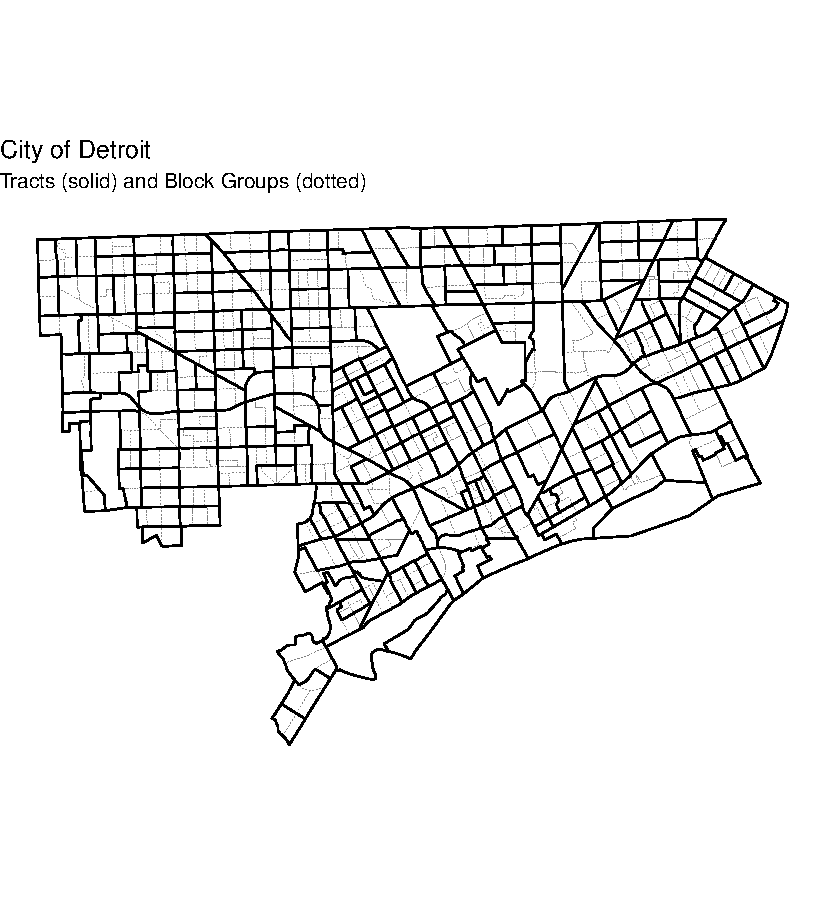
\includegraphics{detroit_sampling_code_files/figure-pdf/fig-fallback-base-1.pdf}

}

\caption{\label{fig-fallback-base}}

\end{figure}%

\begin{Shaded}
\begin{Highlighting}[]
\FunctionTok{ggplot}\NormalTok{() }\SpecialCharTok{+}
  \FunctionTok{geom\_sf}\NormalTok{(}\AttributeTok{data =}\NormalTok{ detroit\_tracts\_sf, }\AttributeTok{fill =} \ConstantTok{NA}\NormalTok{,}
          \AttributeTok{color =} \StringTok{"grey70"}\NormalTok{, }\AttributeTok{linewidth =} \FloatTok{0.3}\NormalTok{) }\SpecialCharTok{+}
  \FunctionTok{geom\_sf}\NormalTok{(}\AttributeTok{data =}\NormalTok{ detroit\_tracts\_sf }\SpecialCharTok{|\textgreater{}} \FunctionTok{filter}\NormalTok{(GEOID }\SpecialCharTok{\%in\%}\NormalTok{ psu\_sample}\SpecialCharTok{$}\NormalTok{Tract),}
          \AttributeTok{fill =} \FunctionTok{viridis}\NormalTok{(}\DecValTok{1}\NormalTok{, }\AttributeTok{begin =} \FloatTok{0.4}\NormalTok{, }\AttributeTok{alpha =} \FloatTok{0.3}\NormalTok{),}
          \AttributeTok{color =} \FunctionTok{viridis}\NormalTok{(}\DecValTok{1}\NormalTok{, }\AttributeTok{begin =} \FloatTok{0.4}\NormalTok{), }\AttributeTok{linewidth =} \FloatTok{0.6}\NormalTok{) }\SpecialCharTok{+}
  \FunctionTok{geom\_sf}\NormalTok{(}\AttributeTok{data =}\NormalTok{ detroit\_bgs\_sf }\SpecialCharTok{|\textgreater{}} \FunctionTok{filter}\NormalTok{(GEOID }\SpecialCharTok{\%in\%}\NormalTok{ sample\_bgs}\SpecialCharTok{$}\NormalTok{BlockGroup),}
          \AttributeTok{fill =} \ConstantTok{NA}\NormalTok{, }\AttributeTok{color =} \StringTok{"red"}\NormalTok{, }\AttributeTok{linewidth =} \FloatTok{0.8}\NormalTok{) }\SpecialCharTok{+}
  \FunctionTok{labs}\NormalTok{(}\AttributeTok{title =} \StringTok{"Selected Sample: 40 Tracts and Block Groups"}\NormalTok{,}
       \AttributeTok{subtitle =} \StringTok{"Blue = sample tracts; Red = selected BGs"}\NormalTok{) }\SpecialCharTok{+}
  \FunctionTok{theme\_void}\NormalTok{(}\AttributeTok{base\_size =} \DecValTok{10}\NormalTok{)}
\end{Highlighting}
\end{Shaded}

\begin{figure}[H]

\centering{

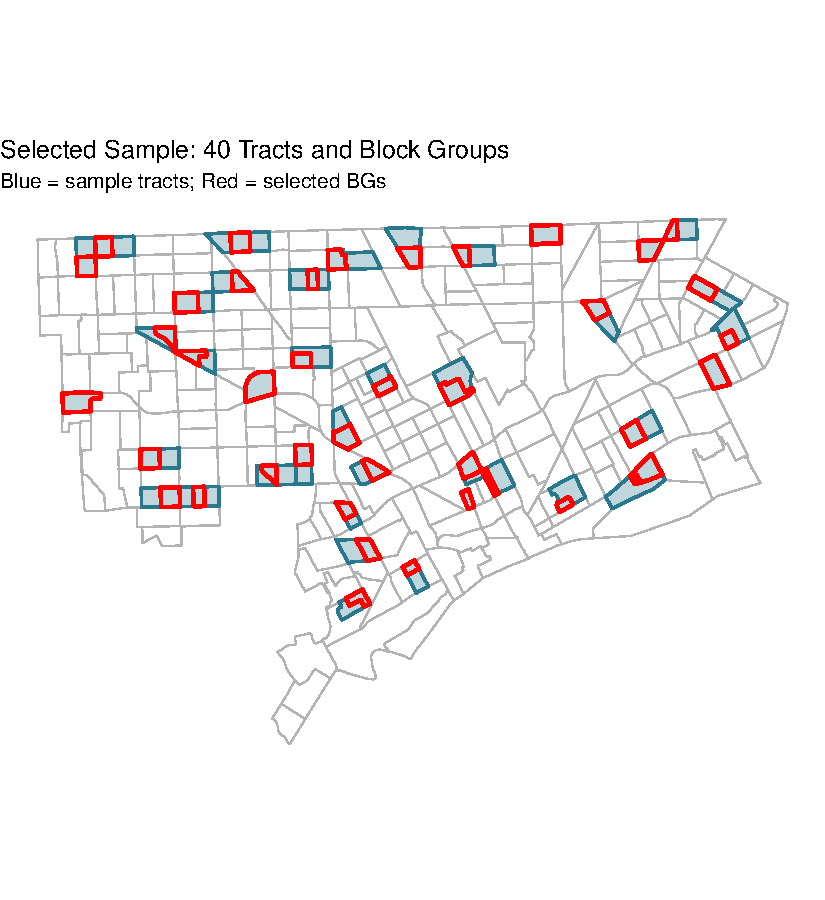
\includegraphics{detroit_sampling_code_files/figure-pdf/fig-fallback-sample-1.pdf}

}

\caption{\label{fig-fallback-sample}}

\end{figure}%

\section{Appendix}\label{sec-appendix}

\subsection{A. Sample PSU and SSU
listing}\label{a.-sample-psu-and-ssu-listing}

\begin{itemize}
\tightlist
\item
  The table below lists all 40 selected BGs with their Census population
  data, composite MOS, selection probabilities at each stage (\(\pi_i\)
  and \(\pi_{j|i}\)), the joint BG probability (\(\pi_{ij}\)), and the
  domain-specific person sampling rates that field teams would
  implement. The rates are listed in the \texttt{rate\_} columns.
\end{itemize}

\begin{Shaded}
\begin{Highlighting}[]
\NormalTok{sample\_listing }\OtherTok{\textless{}{-}}\NormalTok{ sample\_bgs }\SpecialCharTok{|\textgreater{}}
  \FunctionTok{select}\NormalTok{(Tract, BlockGroup, TotAdult, }\FunctionTok{starts\_with}\NormalTok{(}\StringTok{"Age"}\NormalTok{),}
\NormalTok{         MOS\_bg, pi\_i, pij\_given\_i, pi\_ij,}
         \FunctionTok{starts\_with}\NormalTok{(}\StringTok{"rate\_"}\NormalTok{), exp\_workload) }\SpecialCharTok{|\textgreater{}}
  \FunctionTok{arrange}\NormalTok{(Tract)}

\NormalTok{sample\_listing }\SpecialCharTok{|\textgreater{}}
  \FunctionTok{mutate}\NormalTok{(}\FunctionTok{across}\NormalTok{(}\FunctionTok{where}\NormalTok{(is.numeric), }\SpecialCharTok{\textasciitilde{}} \FunctionTok{round}\NormalTok{(.x, }\DecValTok{4}\NormalTok{))) }\SpecialCharTok{|\textgreater{}}
  \FunctionTok{kable}\NormalTok{(}\AttributeTok{n =} \ConstantTok{Inf}\NormalTok{)}
\end{Highlighting}
\end{Shaded}

\begin{longtable}[]{@{}
  >{\raggedright\arraybackslash}p{(\columnwidth - 30\tabcolsep) * \real{0.0723}}
  >{\raggedright\arraybackslash}p{(\columnwidth - 30\tabcolsep) * \real{0.0783}}
  >{\raggedleft\arraybackslash}p{(\columnwidth - 30\tabcolsep) * \real{0.0542}}
  >{\raggedleft\arraybackslash}p{(\columnwidth - 30\tabcolsep) * \real{0.0602}}
  >{\raggedleft\arraybackslash}p{(\columnwidth - 30\tabcolsep) * \real{0.0602}}
  >{\raggedleft\arraybackslash}p{(\columnwidth - 30\tabcolsep) * \real{0.0602}}
  >{\raggedleft\arraybackslash}p{(\columnwidth - 30\tabcolsep) * \real{0.0602}}
  >{\raggedleft\arraybackslash}p{(\columnwidth - 30\tabcolsep) * \real{0.0482}}
  >{\raggedleft\arraybackslash}p{(\columnwidth - 30\tabcolsep) * \real{0.0422}}
  >{\raggedleft\arraybackslash}p{(\columnwidth - 30\tabcolsep) * \real{0.0723}}
  >{\raggedleft\arraybackslash}p{(\columnwidth - 30\tabcolsep) * \real{0.0422}}
  >{\raggedleft\arraybackslash}p{(\columnwidth - 30\tabcolsep) * \real{0.0663}}
  >{\raggedleft\arraybackslash}p{(\columnwidth - 30\tabcolsep) * \real{0.0663}}
  >{\raggedleft\arraybackslash}p{(\columnwidth - 30\tabcolsep) * \real{0.0663}}
  >{\raggedleft\arraybackslash}p{(\columnwidth - 30\tabcolsep) * \real{0.0723}}
  >{\raggedleft\arraybackslash}p{(\columnwidth - 30\tabcolsep) * \real{0.0783}}@{}}
\toprule\noalign{}
\begin{minipage}[b]{\linewidth}\raggedright
Tract
\end{minipage} & \begin{minipage}[b]{\linewidth}\raggedright
BlockGroup
\end{minipage} & \begin{minipage}[b]{\linewidth}\raggedleft
TotAdult
\end{minipage} & \begin{minipage}[b]{\linewidth}\raggedleft
Age18to34
\end{minipage} & \begin{minipage}[b]{\linewidth}\raggedleft
Age35to49
\end{minipage} & \begin{minipage}[b]{\linewidth}\raggedleft
Age50to64
\end{minipage} & \begin{minipage}[b]{\linewidth}\raggedleft
Age65plus
\end{minipage} & \begin{minipage}[b]{\linewidth}\raggedleft
MOS\_bg
\end{minipage} & \begin{minipage}[b]{\linewidth}\raggedleft
pi\_i
\end{minipage} & \begin{minipage}[b]{\linewidth}\raggedleft
pij\_given\_i
\end{minipage} & \begin{minipage}[b]{\linewidth}\raggedleft
pi\_ij
\end{minipage} & \begin{minipage}[b]{\linewidth}\raggedleft
rate\_18\_34
\end{minipage} & \begin{minipage}[b]{\linewidth}\raggedleft
rate\_35\_49
\end{minipage} & \begin{minipage}[b]{\linewidth}\raggedleft
rate\_50\_64
\end{minipage} & \begin{minipage}[b]{\linewidth}\raggedleft
rate\_65plus
\end{minipage} & \begin{minipage}[b]{\linewidth}\raggedleft
exp\_workload
\end{minipage} \\
\midrule\noalign{}
\endhead
\bottomrule\noalign{}
\endlastfoot
26163500200 & 261635002001 & 608 & 211 & 160 & 149 & 88 & 2.7372 &
0.1759 & 0.2888 & 0.0508 & 0.0871 & 0.0965 & 0.0835 & 0.0863 &
53.8614 \\
26163500900 & 261635009001 & 1154 & 427 & 289 & 302 & 136 & 5.1861 &
0.2149 & 0.4477 & 0.0962 & 0.0460 & 0.0509 & 0.0441 & 0.0455 &
53.8614 \\
26163501400 & 261635014002 & 709 & 238 & 185 & 189 & 97 & 3.1886 &
0.2253 & 0.2625 & 0.0592 & 0.0748 & 0.0828 & 0.0717 & 0.0740 &
53.8614 \\
26163502000 & 261635020001 & 1289 & 437 & 357 & 346 & 149 & 5.8076 &
0.1081 & 0.9969 & 0.1077 & 0.0411 & 0.0455 & 0.0394 & 0.0407 &
53.8614 \\
26163503400 & 261635034001 & 673 & 203 & 178 & 190 & 102 & 3.0255 &
0.0563 & 0.9966 & 0.0561 & 0.0788 & 0.0873 & 0.0756 & 0.0780 &
53.8614 \\
26163505200 & 261635052002 & 1496 & 503 & 354 & 352 & 287 & 6.7155 &
0.1839 & 0.6776 & 0.1246 & 0.0355 & 0.0393 & 0.0341 & 0.0352 &
53.8614 \\
26163506100 & 261635061001 & 1379 & 507 & 319 & 336 & 217 & 6.1868 &
0.1148 & 1.0000 & 0.1148 & 0.0385 & 0.0427 & 0.0370 & 0.0382 &
53.8614 \\
26163506900 & 261635069003 & 674 & 213 & 177 & 145 & 139 & 3.0360 &
0.2128 & 0.2647 & 0.0563 & 0.0785 & 0.0870 & 0.0753 & 0.0778 &
53.8614 \\
26163508100 & 261635081002 & 309 & 96 & 81 & 76 & 56 & 1.3904 & 0.0803 &
0.3212 & 0.0258 & 0.1715 & 0.1900 & 0.1645 & 0.1698 & 53.8614 \\
26163511400 & 261635114002 & 843 & 247 & 154 & 230 & 212 & 3.7546 &
0.1391 & 0.5006 & 0.0697 & 0.0635 & 0.0704 & 0.0609 & 0.0629 &
53.8614 \\
26163513900 & 261635139001 & 612 & 169 & 116 & 182 & 145 & 2.7254 &
0.0980 & 0.5160 & 0.0506 & 0.0875 & 0.0969 & 0.0839 & 0.0866 &
53.8614 \\
26163515700 & 261635157001 & 1663 & 551 & 278 & 358 & 476 & 7.4092 &
0.3692 & 0.3723 & 0.1375 & 0.0322 & 0.0357 & 0.0309 & 0.0319 &
53.8614 \\
26163516700 & 261635167001 & 820 & 204 & 107 & 214 & 295 & 3.6296 &
0.2172 & 0.3100 & 0.0673 & 0.0657 & 0.0728 & 0.0630 & 0.0651 &
53.8614 \\
26163517500 & 261635175002 & 1282 & 456 & 178 & 324 & 324 & 5.6876 &
0.2128 & 0.4957 & 0.1055 & 0.0419 & 0.0464 & 0.0402 & 0.0415 &
53.8614 \\
26163520200 & 261635202002 & 2594 & 2492 & 47 & 40 & 15 & 11.4975 &
0.2924 & 0.7296 & 0.2133 & 0.0207 & 0.0230 & 0.0199 & 0.0205 &
53.8614 \\
26163521800 & 261635218001 & 1179 & 282 & 207 & 249 & 441 & 5.2540 &
0.0975 & 1.0000 & 0.0975 & 0.0454 & 0.0503 & 0.0435 & 0.0449 &
53.8614 \\
26163523300 & 261635233001 & 639 & 236 & 218 & 124 & 61 & 2.9078 &
0.1709 & 0.3156 & 0.0539 & 0.0820 & 0.0908 & 0.0786 & 0.0812 &
53.8614 \\
26163524200 & 261635242003 & 1144 & 434 & 356 & 255 & 99 & 5.1839 &
0.2349 & 0.4095 & 0.0962 & 0.0460 & 0.0510 & 0.0441 & 0.0455 &
53.8614 \\
26163525700 & 261635257001 & 946 & 349 & 304 & 198 & 95 & 4.2931 &
0.2449 & 0.3253 & 0.0796 & 0.0555 & 0.0615 & 0.0533 & 0.0550 &
53.8614 \\
26163526400 & 261635264002 & 458 & 162 & 121 & 108 & 67 & 2.0628 &
0.0803 & 0.4768 & 0.0383 & 0.1156 & 0.1281 & 0.1109 & 0.1145 &
53.8614 \\
26163530800 & 261635308001 & 648 & 173 & 141 & 198 & 136 & 2.8942 &
0.0914 & 0.5873 & 0.0537 & 0.0824 & 0.0913 & 0.0790 & 0.0816 &
53.8614 \\
26163531800 & 261635318002 & 551 & 158 & 116 & 169 & 108 & 2.4593 &
0.0945 & 0.4826 & 0.0456 & 0.0969 & 0.1074 & 0.0930 & 0.0960 &
53.8614 \\
26163533600 & 261635336001 & 438 & 130 & 106 & 123 & 79 & 1.9639 &
0.0864 & 0.4219 & 0.0364 & 0.1214 & 0.1345 & 0.1164 & 0.1202 &
53.8614 \\
26163534700 & 261635347003 & 887 & 270 & 205 & 250 & 162 & 3.9723 &
0.1851 & 0.3981 & 0.0737 & 0.0600 & 0.0665 & 0.0576 & 0.0594 &
53.8614 \\
26163535600 & 261635356001 & 531 & 133 & 114 & 152 & 132 & 2.3719 &
0.2424 & 0.1815 & 0.0440 & 0.1005 & 0.1114 & 0.0964 & 0.0995 &
53.8614 \\
26163536400 & 261635364001 & 660 & 194 & 177 & 148 & 141 & 2.9734 &
0.1347 & 0.4097 & 0.0552 & 0.0802 & 0.0888 & 0.0769 & 0.0794 &
53.8614 \\
26163537200 & 261635372001 & 450 & 122 & 131 & 126 & 71 & 2.0288 &
0.0377 & 0.9974 & 0.0376 & 0.1175 & 0.1302 & 0.1127 & 0.1164 &
53.8614 \\
26163538200 & 261635382001 & 905 & 193 & 222 & 222 & 268 & 4.0606 &
0.1366 & 0.5514 & 0.0753 & 0.0587 & 0.0651 & 0.0563 & 0.0581 &
53.8614 \\
26163538600 & 261635386001 & 963 & 250 & 248 & 273 & 192 & 4.3238 &
0.2995 & 0.2678 & 0.0802 & 0.0551 & 0.0611 & 0.0529 & 0.0546 &
53.8614 \\
26163539200 & 261635392003 & 1517 & 437 & 325 & 402 & 353 & 6.7827 &
0.3243 & 0.3880 & 0.1258 & 0.0352 & 0.0389 & 0.0337 & 0.0348 &
53.8614 \\
26163539600 & 261635396001 & 1050 & 329 & 224 & 291 & 206 & 4.6936 &
0.2028 & 0.4293 & 0.0871 & 0.0508 & 0.0563 & 0.0487 & 0.0503 &
53.8614 \\
26163540400 & 261635404002 & 962 & 258 & 215 & 286 & 203 & 4.3008 &
0.1696 & 0.4704 & 0.0798 & 0.0554 & 0.0614 & 0.0532 & 0.0549 &
53.8614 \\
26163540900 & 261635409002 & 1158 & 343 & 256 & 265 & 294 & 5.1879 &
0.2199 & 0.4377 & 0.0962 & 0.0460 & 0.0509 & 0.0441 & 0.0455 &
53.8614 \\
26163541500 & 261635415001 & 1352 & 373 & 289 & 378 & 312 & 6.0412 &
0.2403 & 0.4665 & 0.1121 & 0.0395 & 0.0437 & 0.0379 & 0.0391 &
53.8614 \\
26163542300 & 261635423001 & 667 & 217 & 161 & 149 & 140 & 2.9966 &
0.1462 & 0.3802 & 0.0556 & 0.0796 & 0.0882 & 0.0763 & 0.0788 &
53.8614 \\
26163543000 & 261635430001 & 695 & 189 & 166 & 154 & 186 & 3.1200 &
0.1183 & 0.4895 & 0.0579 & 0.0764 & 0.0847 & 0.0733 & 0.0757 &
53.8614 \\
26163544000 & 261635440001 & 1985 & 694 & 473 & 568 & 250 & 8.8996 &
0.1625 & 1.0159 & 0.1651 & 0.0268 & 0.0297 & 0.0257 & 0.0265 &
53.8614 \\
26163545500 & 261635455001 & 835 & 308 & 231 & 196 & 100 & 3.7669 &
0.2186 & 0.3196 & 0.0699 & 0.0633 & 0.0701 & 0.0607 & 0.0627 &
53.8614 \\
26163545900 & 261635459002 & 1248 & 524 & 333 & 283 & 108 & 5.6278 &
0.2140 & 0.4878 & 0.1044 & 0.0424 & 0.0469 & 0.0406 & 0.0420 &
53.8614 \\
26163546700 & 261635467001 & 1268 & 433 & 279 & 319 & 237 & 5.6785 &
0.1746 & 0.6033 & 0.1053 & 0.0420 & 0.0465 & 0.0403 & 0.0416 &
53.8614 \\
\end{longtable}

\subsection{B. Export files}\label{b.-export-files}

\begin{Shaded}
\begin{Highlighting}[]
\CommentTok{\# uncomment when paths are configured}
\CommentTok{\# write\_csv(psu\_frame, here("paper", "FRAME\_PSU\_EffectSize.csv"))}
\CommentTok{\# write\_csv(ssu\_frame, here("paper", "FRAME\_BG\_EffectSize.csv"))}
\CommentTok{\# write\_csv(sample\_listing, here("paper", "SAMPLE\_EffectSize.csv"))}
\end{Highlighting}
\end{Shaded}

\subsection{C. AI disclosure}\label{c.-ai-disclosure}

This project utilized \textbf{Claude (Anthropic, Opus 4.6)} for code
development, report drafting, and cross-checking calculations against
VDK textbook formulas and lecture slide materials. All AI outputs were
reviewed, verified against source materials, and modified by team
members before inclusion.




\end{document}
